% Nature Physics initial-submission version of paper/draft_v1p1_prl.tex.
% Springer Nature template v3.1 (December 2024), Nature Portfolio option.
\documentclass[pdflatex,sn-nature]{sn-jnl}
\usepackage{graphicx,xcolor}
\usepackage{amsmath,amssymb}
\geometry{reset,a4paper,margin=20mm}
\hypersetup{hidelinks,pdftitle={Blast freezing a black hole}}
\unnumbered
\raggedbottom
\begin{document}
\title{Blast freezing a black hole}
\author*[1]{\fnm{Shoaib} \sur{Akhtar}}\email{shoaib@stanford.edu}
\author*[1,2]{\fnm{Xiao-Liang} \sur{Qi}}\email{xlqi@stanford.edu}
\affil[1]{\orgname{Leinweber Institute for Theoretical Physics, Stanford University}, \orgaddress{\city{Stanford}, \state{CA}, \postcode{94305}, \country{USA}}}
\affil[2]{\orgname{OpenAI}}
\abstract{What happens to information carried through an evaporating black-hole horizon? We introduce a solvable model of evaporation built from coupled Sachdev-Ye-Kitaev systems, in which an initially two-sided black hole is coupled at a finite time to a larger, colder bath. Evaporation is rapid in this model, so we refer to the process as ``blast freezing'' of a black hole. In an appropriate large-$N$ and large-$p$ limit, the two-point functions and certain four-point probes can be computed analytically. Using the two-point functions as input to a generalized HKLL reconstruction, we obtain the emergent bulk geometry of the evaporation process. We then track the information carried by an infalling particle using operator size and Renyi-2 mutual information, showing how it is preserved in nonlocal many-body degrees of freedom after the blast-freezing transition.}
\maketitle

\section{Black-hole information and evaporation}

One of the deepest open questions in science is how to unify the two pillars of modern physics: quantum mechanics and general relativity. Black holes sharpen this tension. Quantum mechanics predicts unitary time evolution, while classical general relativity predicts that the black hole horizon is a one-way surface that information enters and never leaves. This is known as the black hole information paradox. There are different types of information paradoxes. The ``old'' paradox proposed by Hawking\cite{hawking1976breakdown} concerns the fate of infalling information after the black hole evaporates: quantum mechanics says it should be preserved in the Hawking radiation, whereas the semiclassical radiation appears thermal. This paradox is resolved by a modified gravitational path integral approach\cite{penington2020entanglement,penington2022replica,almheiri2019entropy,almheiri2020replica}. However, the firewall paradox\cite{almheiri2013black,almheiri2013apologia}, which concerns the experience of an infalling observer, remains open. General relativity predicts that the observer feels nothing special when crossing the horizon, while quantum mechanics predicts that, at a late enough time, information in the interior is already known to the exterior Hawking radiation. If an interior particle is completely entangled with a nearby partner, it cannot also be entangled with the radiation, so the local quantum field theory description appears to fail. To resolve this paradox, a more explicit description of quantum dynamics in the black hole interior is needed.

\begin{figure}[htbp]
	\centering
	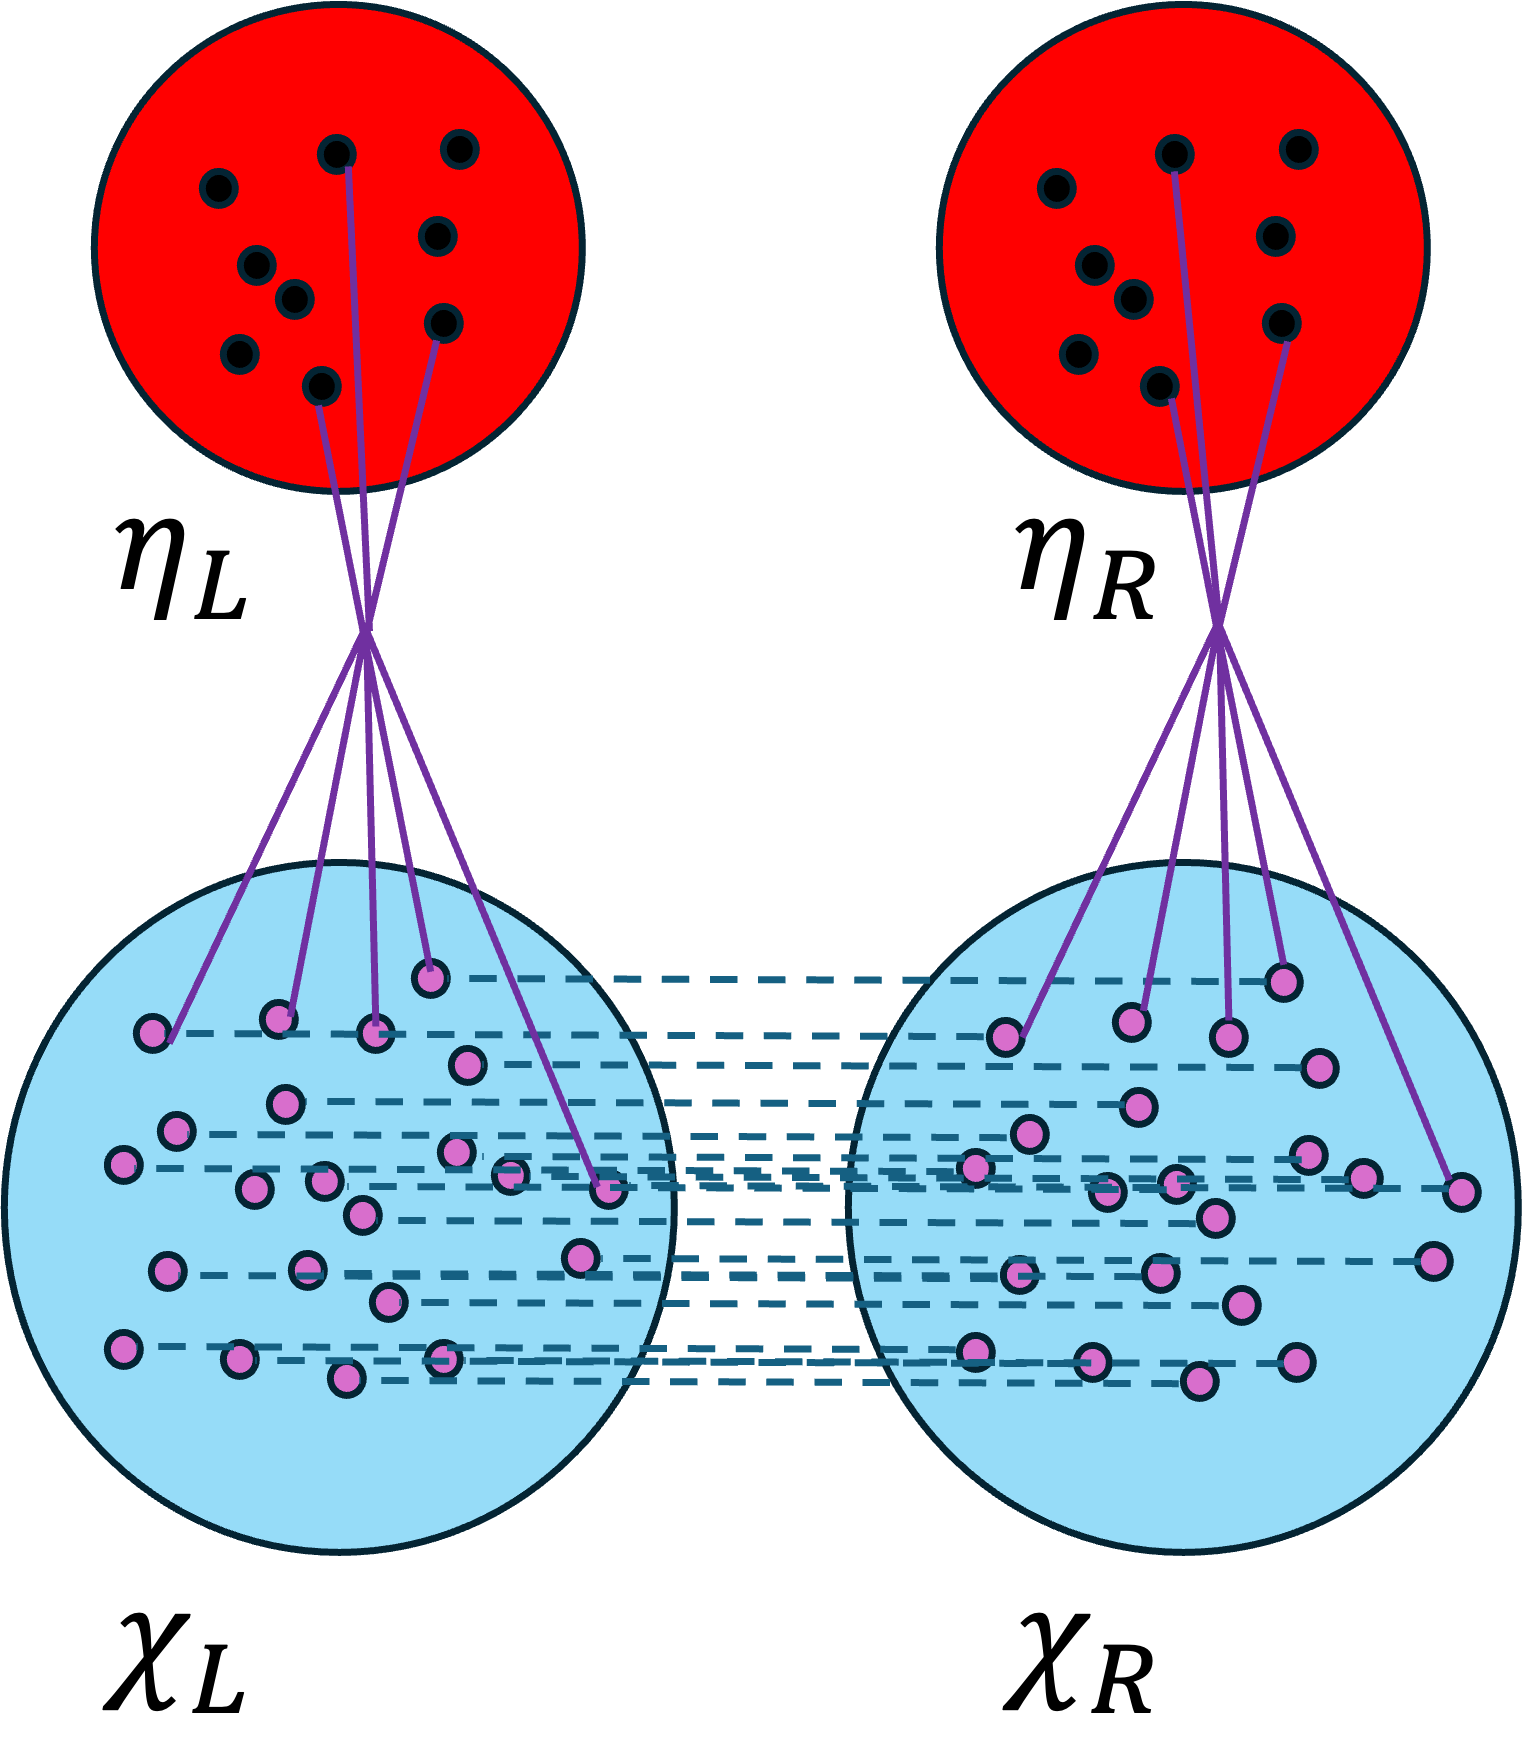
\includegraphics[width=0.30\textwidth]{fig1.png}
	\caption{Illustration of the model setup. The dashed lines illustrate the bilinear coupling between $\chi$ fermions, while the solid lines illustrate the SYK coupling between $\eta$ and $\chi$ fermions, which is only turned on after the evaporation time $t_{\rm ev}$.}\label{fig:setup}
\end{figure}

In this paper, we provide new insight into the black hole information paradox by proposing a new model of a $1+1$-dimensional evaporating black hole. Our proposal is based on holographic duality, also known as the Anti-de Sitter/Conformal field theory (AdS/CFT) correspondence\cite{maldacena1999large}. Holographic duality is the mapping between a theory of gravity in $d+1$ dimensional spacetime and a quantum field theory in $d$ dimensional spacetime.
The Sachdev-Ye-Kitaev (SYK) model\cite{sachdev1993gapless,kitaev2015simple,maldacena2016remarks} is proposed as a $d=0$ example of this duality, where the boundary model describes $N$ interacting Majorana fermions, and the dual bulk theory is $1+1$-d Jackiw-Teitelboim (JT) gravity\cite{jackiw1985lower,teitelboim1983gravitation} (coupled with matter fields). In holographic duality, a thermal state of the boundary theory corresponds to a black hole in the bulk theory. Thermal correlation functions of fermions in the low temperature SYK model are reproduced by the fermion two-point function in the background of a $1+1$-dimensional AdS black hole. However, large black holes in AdS space do not evaporate, so to study black hole evaporation, we need to couple the SYK model to a bath system. The model we consider contains four SYK islands (Fig. \ref{fig:setup}). Two of them are entangled in a thermal-field double state of $N_\eta$ Majorana fermions $\eta_{iL},\eta_{iR}$, but they are not coupled. The other two islands each contain $N_\chi$ Majorana fermions $\chi_{iL},\chi_{iR}$. We consider $\eta$ fermions as a model of the black hole and the $\chi$ fermions as a model of the bath, so we are interested in the region $N_\chi >N_\eta$. The $\chi$ fermions are coupled by a bilinear coupling, which defines a Hamiltonian with a unique ground state and gapped excitations. It was shown that\cite{maldacena2018eternal} ground state physics in this coupled system is dual to a global AdS$_2$ geometry, which provides a good candidate for a cool bath system. Then we turn on a coupling between $\eta$ and $\chi$ fermions at some finite time $t_{\rm ev}$. The coupling leads to a transfer of energy and entropy from $\eta$ fermions to the cooler $\chi$ fermion system, which describes the black hole evaporation process. We will show that this model is solvable in the large $N_\eta,N_\chi$ limit. In particular, when all SYK islands have $p$-body interactions and \(s=N_\eta/(N_\eta+N_\chi)\), we consider the limit $p\rightarrow \infty, N_\eta\rightarrow \infty, N_\chi\rightarrow \infty, p^2/N_\eta\rightarrow 0, sp\rightarrow 0$. In this limit two-point functions can be solved analytically, which enables us to study many aspects of this model and its gravity dual. By applying the bulk reconstruction algorithm developed in Ref.\cite{nebabu2024bulk}, we obtain the $1+1$-d bulk fermion dynamics and the infalling bulk operators. We analyze the bulk geometry and show how the $\eta$ fermion experiences a quick transition from the black hole geometry to a vacuum with an end-of-the-world brane. This analytic solution also allows us to obtain further information about the fate of infalling operators at the horizon, which provides some new insight about the black hole information paradox. Similar models of the SYK model coupled with a bath have been studied before\cite{zhang2019evaporation,chen2020replica,gaikwad2023microscopic,bragagnolo2026probing}, but bulk reconstruction in such models has not been constructed from the boundary theory.

In the following, we will first define the model and then introduce its key properties.

\section{Definition of the Model}
The model we study has the following Hamiltonian:
\begin{equation}
H_{\rm tot}(t)=H^L+H^R
+i\frac{\mu_\eta(t)}{p}\sum_{k=1}^{N_\eta}\eta_{Lk}\eta_{Rk}
+i\frac{\mu_\chi(t)}{p}\sum_{k=1}^{N_\chi}\chi_{Lk}\chi_{Rk}.
\end{equation}
where $H^R=H[\eta^R,\chi^R]$ and $H^L=(-1)^{p/2}H[\eta^L,\chi^L]$ are time-dependent Hamiltonians, each of which describes two independent SYK islands that are merged into one bigger SYK island at time $t=t_{\rm ev}$. More precisely,
\begin{align}
	H[\eta,\chi]=\left\{\begin{array}{cc}H_{\rm SYK}[\eta]+H_{\rm SYK}[\chi],&t<t_{\rm ev}\\
										H_{\rm SYK}[\eta\oplus \chi],&t\geq t_{\rm ev}\end{array}\right.
\end{align}
Here $H_{\rm SYK}[\eta\oplus \chi]$ means we treat the $N_\eta+N_\chi$ fermions $\eta$ and $\chi$ together as a bigger SYK island. More details about the model definition are provided in Methods and Supplementary Text, Sec.~S1. The bilinear coupling distinguishes $\eta$ and $\chi$ dynamics. In most of the paper, we will consider $\mu_\eta(t)\equiv 0$ so that the $\eta$ fermions are in a two-sided black hole state before they are coupled with $\chi$, while $\mu_\chi(t)=\mu_0$ is a constant which allows the $\chi$ fermions to be in the traversable wormhole phase\cite{maldacena2018eternal}. Before the coupling is turned on, the $\eta$ fermions are in a time-evolved thermal field double state, which in the energy eigenstate basis has the form $\left|TFD(t)\right\rangle=Z_\beta^{-1/2}\sum_n e^{-\beta E_n/2}e^{-2iE_nt}\left|n\right\rangle_L\left|n\right\rangle_R$. The $\chi$ fermions are in the ground state of the traversable wormhole.

\section{The solvable limit}
We first take the large $N$ limit
\begin{align}
N_\eta\rightarrow \infty,\quad N_\chi\rightarrow \infty,\quad s=\frac{N_\eta}{N_\eta+N_\chi}={\rm const}.
\end{align}
In this limit, the dynamics of the system can be described by the Kadanoff-Baym (KB) equation, which is a self-consistent equation for the two-point functions of $\eta$ and $\chi$ fermions. For a simple SYK site, the self-energy is determined by its two-point function. Schematically $\Sigma\propto \mathcal{J}^2G^{p-1}$. In our model, the self-energy becomes a weighted sum of $G_\eta^kG_{\chi}^{p-1-k}$ kinds of terms, with a time-dependent weight.

Details about the KB equations are summarized in Methods and derived in Supplementary Text, Sec.~S2. Here we specialize to the simplest limit that retains the essential physics of black-hole evaporation:
\begin{align}
p\rightarrow \infty,\quad \frac{p^2}{N_\eta}\rightarrow 0,\quad sp\rightarrow 0
\end{align}
This is the large bath limit when $N_\chi \gg N_\eta p$. In this limit, the effect of $\chi$ fermions dominates the $\eta$ self-energy, while the back-reaction of $\eta$ fermions on $\chi$ fermions is negligible. This allows us to generalize the large-$p$ solution of the SYK model\cite{maldacena2016remarks}. In this limit, the two-point function has the following form:
\begin{displaymath}
	G^{\psi,>}(t_1,t_2)=-\frac{1}{2}
	\left(\begin{array}{cc}
	i e^{g^\psi_R(t_1,t_2)/p} & e^{g^\psi_L(t_1,t_2)/p}\\
	-e^{g^\psi_L(t_1,t_2)/p} & +i e^{g^\psi_R(t_1,t_2)/p}
	\end{array}\right).
\end{displaymath}
Here $\psi$ represents $\eta$ or $\chi$ fermions. The KB equation reduces to differential equations for $g^\psi_{L,R}$. $g^\chi_{R,L}$ satisfies the Liouville equation, which is the same as a stand-alone large-$p$ solution:
\begin{align}
	 \partial_{t_1}\partial_{t_2}g^\chi_{R,L}=\pm 2\mathcal{J}^2e^{g^\chi_{R,L}}\label{eq:large_p_chi}
\end{align}
For $\eta$ fermions, the right-hand side is a bit more complicated:
\begin{equation}
\partial_{t_1}\partial_{t_2}g^\eta_{R,L}=\left\{\begin{array}{cc}\pm2\mathcal{J}^2e^{g^\eta_{R,L}},&t_1,t_2<t_{\rm ev}\\\pm2\mathcal{J}^2e^{g^\chi_{R,L}},&t_1,t_2>t_{\rm ev}\\0,&\text{otherwise}\end{array}\right.\label{eq:large_p_eta}
\end{equation}
This equation illustrates that the self-energy of $\eta$ fermions is entirely determined by $\chi$ after the evaporation time. Furthermore, the self-energy becomes block-diagonal: the self-energy between the $t<t_{\rm ev}$ region and the $t>t_{\rm ev}$ region vanishes. Both are consequences of the fact that the most important terms in the Hamiltonian switched from $\eta^p$ types of terms to $\eta\chi^{p-1}$ types of terms. The solution of the $\chi$ equation has been studied before for generic couplings $\mu_\chi(t)$ with a thermal field double initial state\cite{lensky2021rescuing}. The $\eta$ equation (\ref{eq:large_p_eta}) can also be solved.

The probe-limit solutions for \(g^\chi\) and \(g^\eta\), including their matching across \(t_{\rm ev}\), are summarized in Methods and derived in Supplementary Text, Sec.~S3. The two-point function has the form
\begin{align}
g^\eta_{R(L)}(t_1,t_2)
&=f_{1R(L)}(t_1)+f_{2R(L)}(t_2),
\quad t_2<t_{\rm ev}<t_1,\label{eq:regionII}\\
g^\eta_{R(L)}(t_1,t_2)
&=g^\chi_{R,L}(t_1,t_2)+f_{3R(L)}(t_1)+f^*_{3R(L)}(t_2),
\quad t_1,t_2>t_{\rm ev}.\label{eq:regionIII}
\end{align}
With the ordering shown in Eq.~\eqref{eq:regionII}, \(f_2\) is fixed by the pre-evaporation $\eta$ solution, while \(f_1\) and \(f_3\) are fixed by the post-evaporation $\chi$ evolution.

The form of Eq. (\ref{eq:regionII}) has a deep consequence. The two-point function has the factorized form $e^{g^\eta_{R(L)}(t_1,t_2)/p}=e^{f_{1R(L)}(t_1)/p}e^{f_{2R(L)}(t_2)/p}$ in the region $t_2<t_{\rm ev}<t_1$. Consider the linear spaces $\mathbb{V}_{\rm past}$ spanned by $\eta(t),t<t_{\rm ev}$ and $\mathbb{V}_{\rm fut}$ spanned by $\eta(t),t>t_{\rm ev}$. The overlap between these two spaces is defined by the expectation value of the anti-commutator, $A_{ab}(t_1,t_2)=\langle\{\eta_a(t_1),\eta_b(t_2)\}\rangle=-2\operatorname{Im}G^{\eta,>}_{ab}(t_1,t_2)$ (Supplementary Text, Sec.~S3). It has rank $\leq4$ per flavor due to the factorized correlator. This means that the single particle states from the past are almost orthogonal to those detectable in the future, except at most four independent modes per flavor. This is consistent with the fact that information that falls into the black hole in the form of simple states appears to be lost in the large $N$ limit. When we consider finite $N$ effects, we see that such information actually returns in complex operators, which will be discussed below.
We believe this is the first black hole evaporation model where the information loss in the large-$N$ limit is analytically tractable from a boundary calculation.

\section{Bulk Reconstruction}

To turn such intuition into sharp quantitative statements, we would like to study the holographic dual of this model. In the large $N$ limit, $\eta$ is a generalized free field, and we can apply the bulk reconstruction algorithm developed in Refs.~\cite{nebabu2024bulk,nebabu2026two}. The algorithm constructs a $1+1$-d bulk free fermion theory with the boundary correlators identical to the boundary Wightman function \(C_{ab}(t_1,t_2)=\left\langle \eta_a(t_1)\eta_b(t_2)\right\rangle\). Importantly, up to a local basis choice, the bulk theory is uniquely determined by the boundary Wightman function. The bulk fermion is related to the boundary fermion by a linear kernel, which is a generalization of the Hamilton-Kabat-Lifschytz-Lowe (HKLL) construction\cite{hamilton2006holographic}. The boundary anti-commutator defines the inner product on the linear space of simple boundary operators, and the bulk reconstruction kernel is determined by the requirement of canonical anti-commutation relations for the bulk fermions. In general, this procedure has to be implemented numerically, but
analytic results can be obtained for a large class of time-translation invariant correlation functions\cite{nebabu2026two}. Interestingly, the reconstruction does not refer to an AdS background, and the bulk geometry obtained may have either sign of curvature. As a special case, this algorithm correctly reproduces the duality between the low temperature SYK model and AdS$_2$ geometry. Details of the construction are given in Methods.

\begin{figure}[htbp]
	\centering
	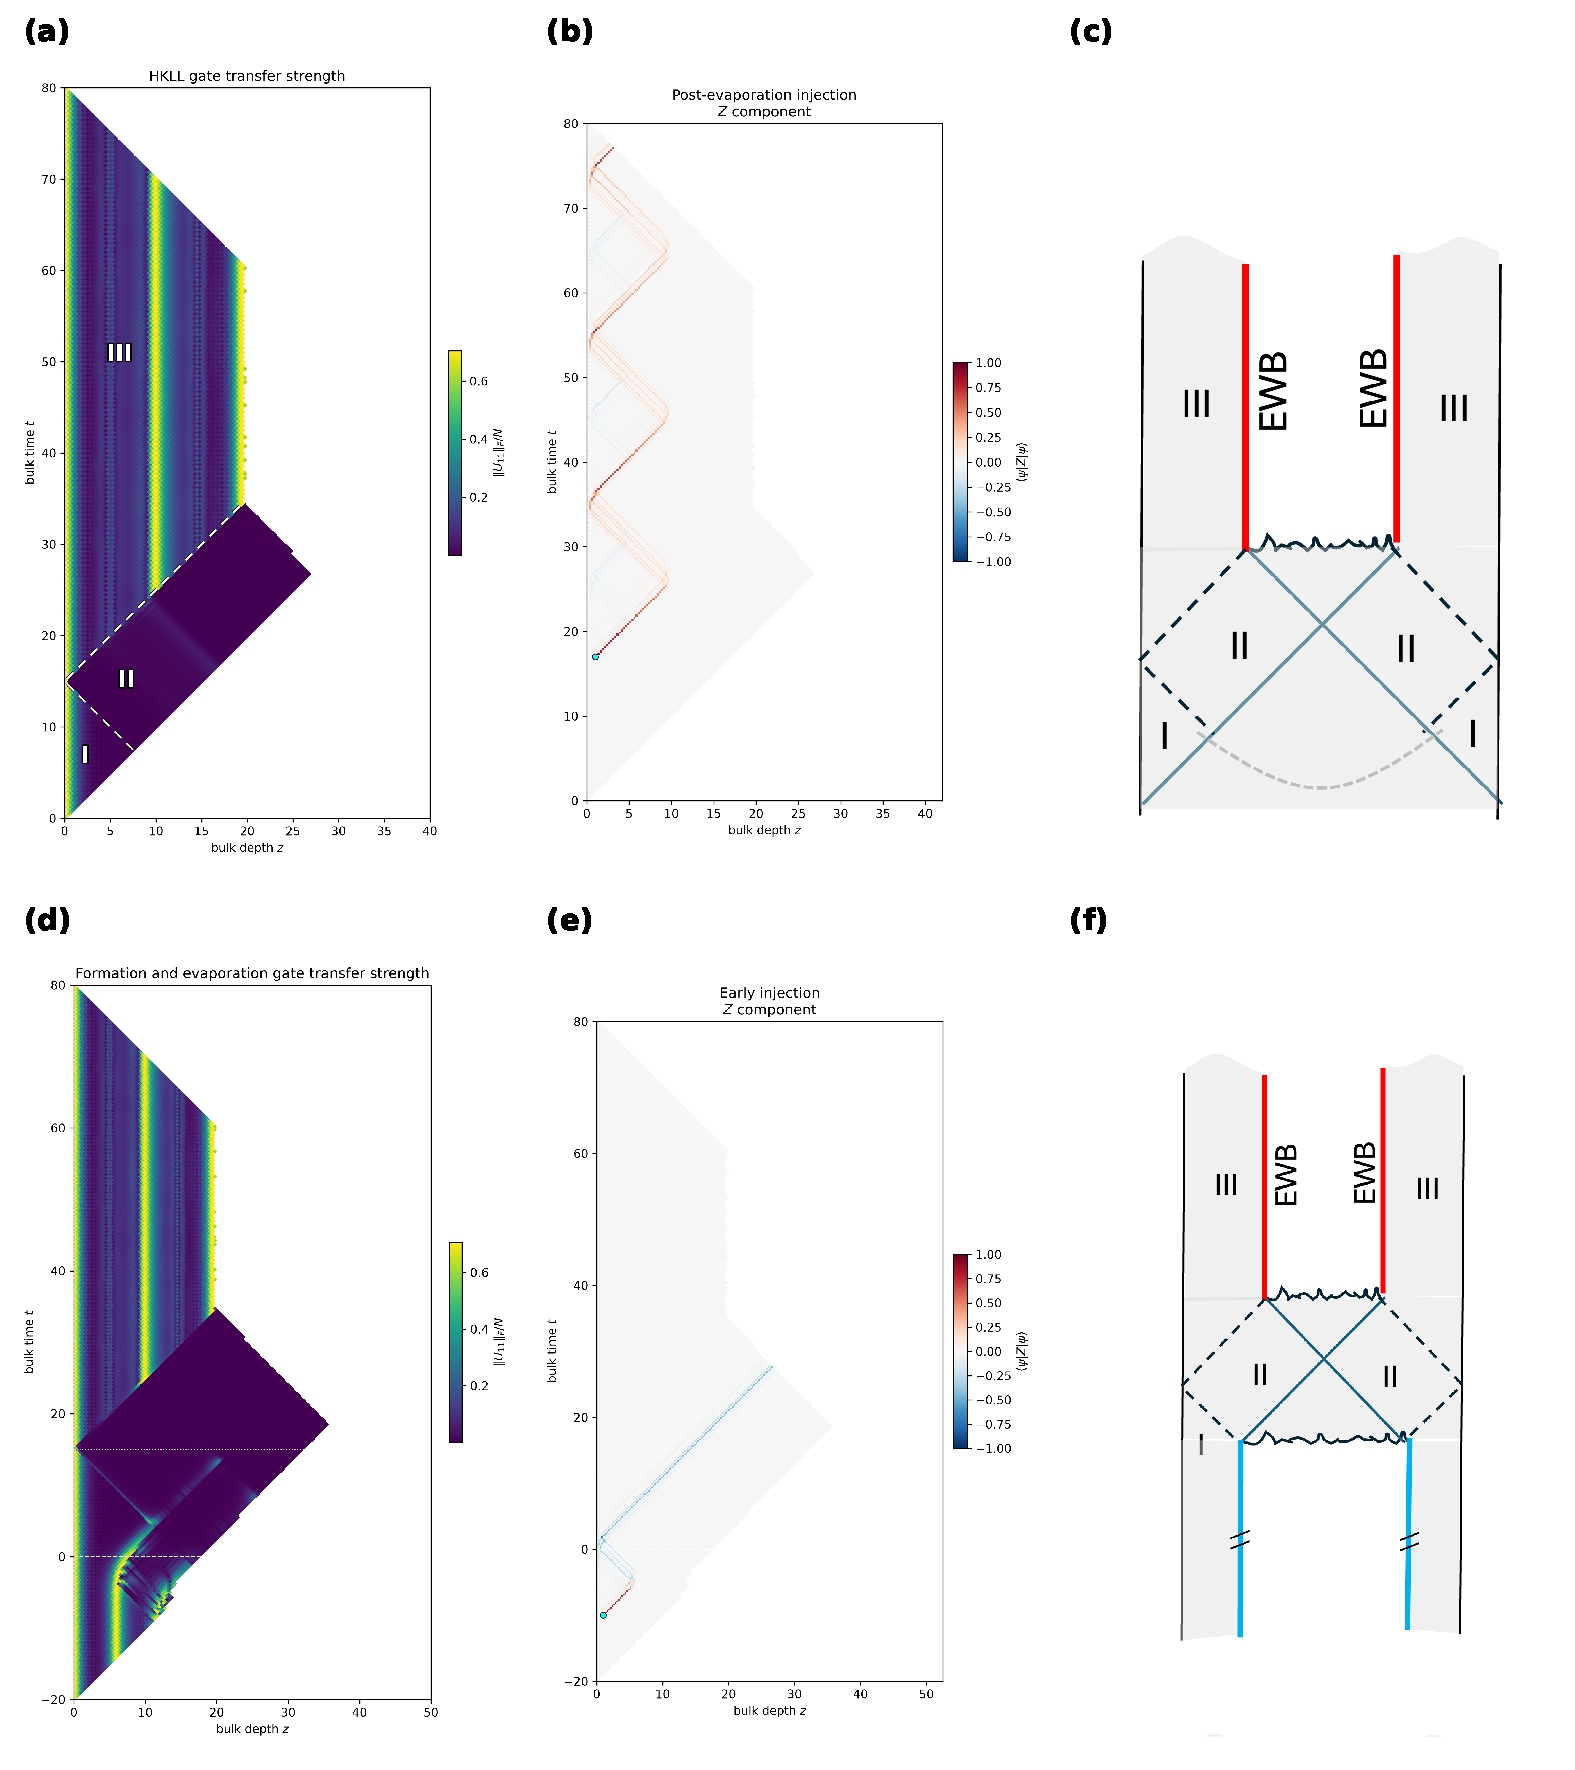
\includegraphics[width=\textwidth]{figure2_bulk_geometry.pdf}
	\caption{Bulk reconstruction of the blast freezing model. The color map in (a) represents reflection probability at the bulk coordinate $(u,v)$ when the state before evaporation is an eternal black hole. (b) shows the propagation of a wavepacket in this geometry when a particle is sent in after evaporation. The color is the polarization in the L, R components. The figure shows that a particle from the left does not reach the right boundary. (c) is the unfolded Penrose diagram illustration based on the results in (a) and (b). (d), (e), and (f) are the same plots for a different state. The initial state was a traversable wormhole and a black hole is formed at $t=0$.}\label{fig:bulk_geometry}
\end{figure}

One interesting aspect of this reconstruction algorithm that is relevant to the current work is that the boundary anti-commutator determines not only the bulk geometry but also its topology. When the anti-commutator matrix on a boundary time interval becomes singular, further expanding the interval does not generate new orthogonal bulk modes, and the reconstructed geometry ends. Applying this reconstruction algorithm to $\eta_a(t)$ fermions in our model leads to the geometry of Fig.~\ref{fig:bulk_geometry} (a). (Parameters used to plot all figures are provided in the last subsection of Methods.) Region I corresponds to the two-sided black hole geometry, region II to the transition region, and region III to the geometry after evaporation. Because the post-evaporation $\eta$ correlator inherits the oscillatory bath dynamics, the reconstructed geometry ends at finite depth. However, unlike the $\chi$ traversable wormhole, the $\eta$ geometry does not connect the left and right boundaries with appreciable probability. The evolution of a fermion wavepacket in Fig.~\ref{fig:bulk_geometry} (b) shows that the color never changes from red to blue, which implies that the left-boundary fermion never propagates to the right boundary. This is consistent with the analytic left-right correlator bound derived in Supplementary Text, Secs.~S3 and S6. Physically, this is because the coupling with $\chi$ cannot restore the already scrambled left-right correlation of $\eta$. Schematically, the unfolded geometry looks like Fig.~\ref{fig:bulk_geometry} (c), with a pair of end-of-the-world branes.

To obtain a more complete picture of the black hole evaporation procedure, we can also introduce a black hole formation process before the evaporation. This can be achieved by considering a nonzero constant $\mu_\eta$ bilinear coupling for $t<0$. At time $t=0$ we turn off the coupling, which corresponds to an in-falling light-like shell of matter that creates a black hole. Then at a later time $t_{\rm ev}$ we turn on the coupling with the bath. In this case, the bulk geometry has an unusual topology illustrated in Fig.~\ref{fig:bulk_geometry} (d-f). If no bath coupling is introduced, the geometry is a traversable wormhole turning into a black hole (which can be verified by the wavepacket propagation picture in subfigure (e)), with a future horizon but no past horizon. The coupling with the bath requires a modified geometry with both a future horizon and a past horizon. Physically we can consider the modes at the past horizon as auxiliary degrees of freedom which are introduced to represent the effect of the bath. It is interesting to note that a similar spacetime geometry has been discussed but then excluded for a different type of model that couples JT gravity with a bath\cite{almheiri2025}.

\section{Fate of Infalling Information}

\begin{figure}[htbp]
	\centering
	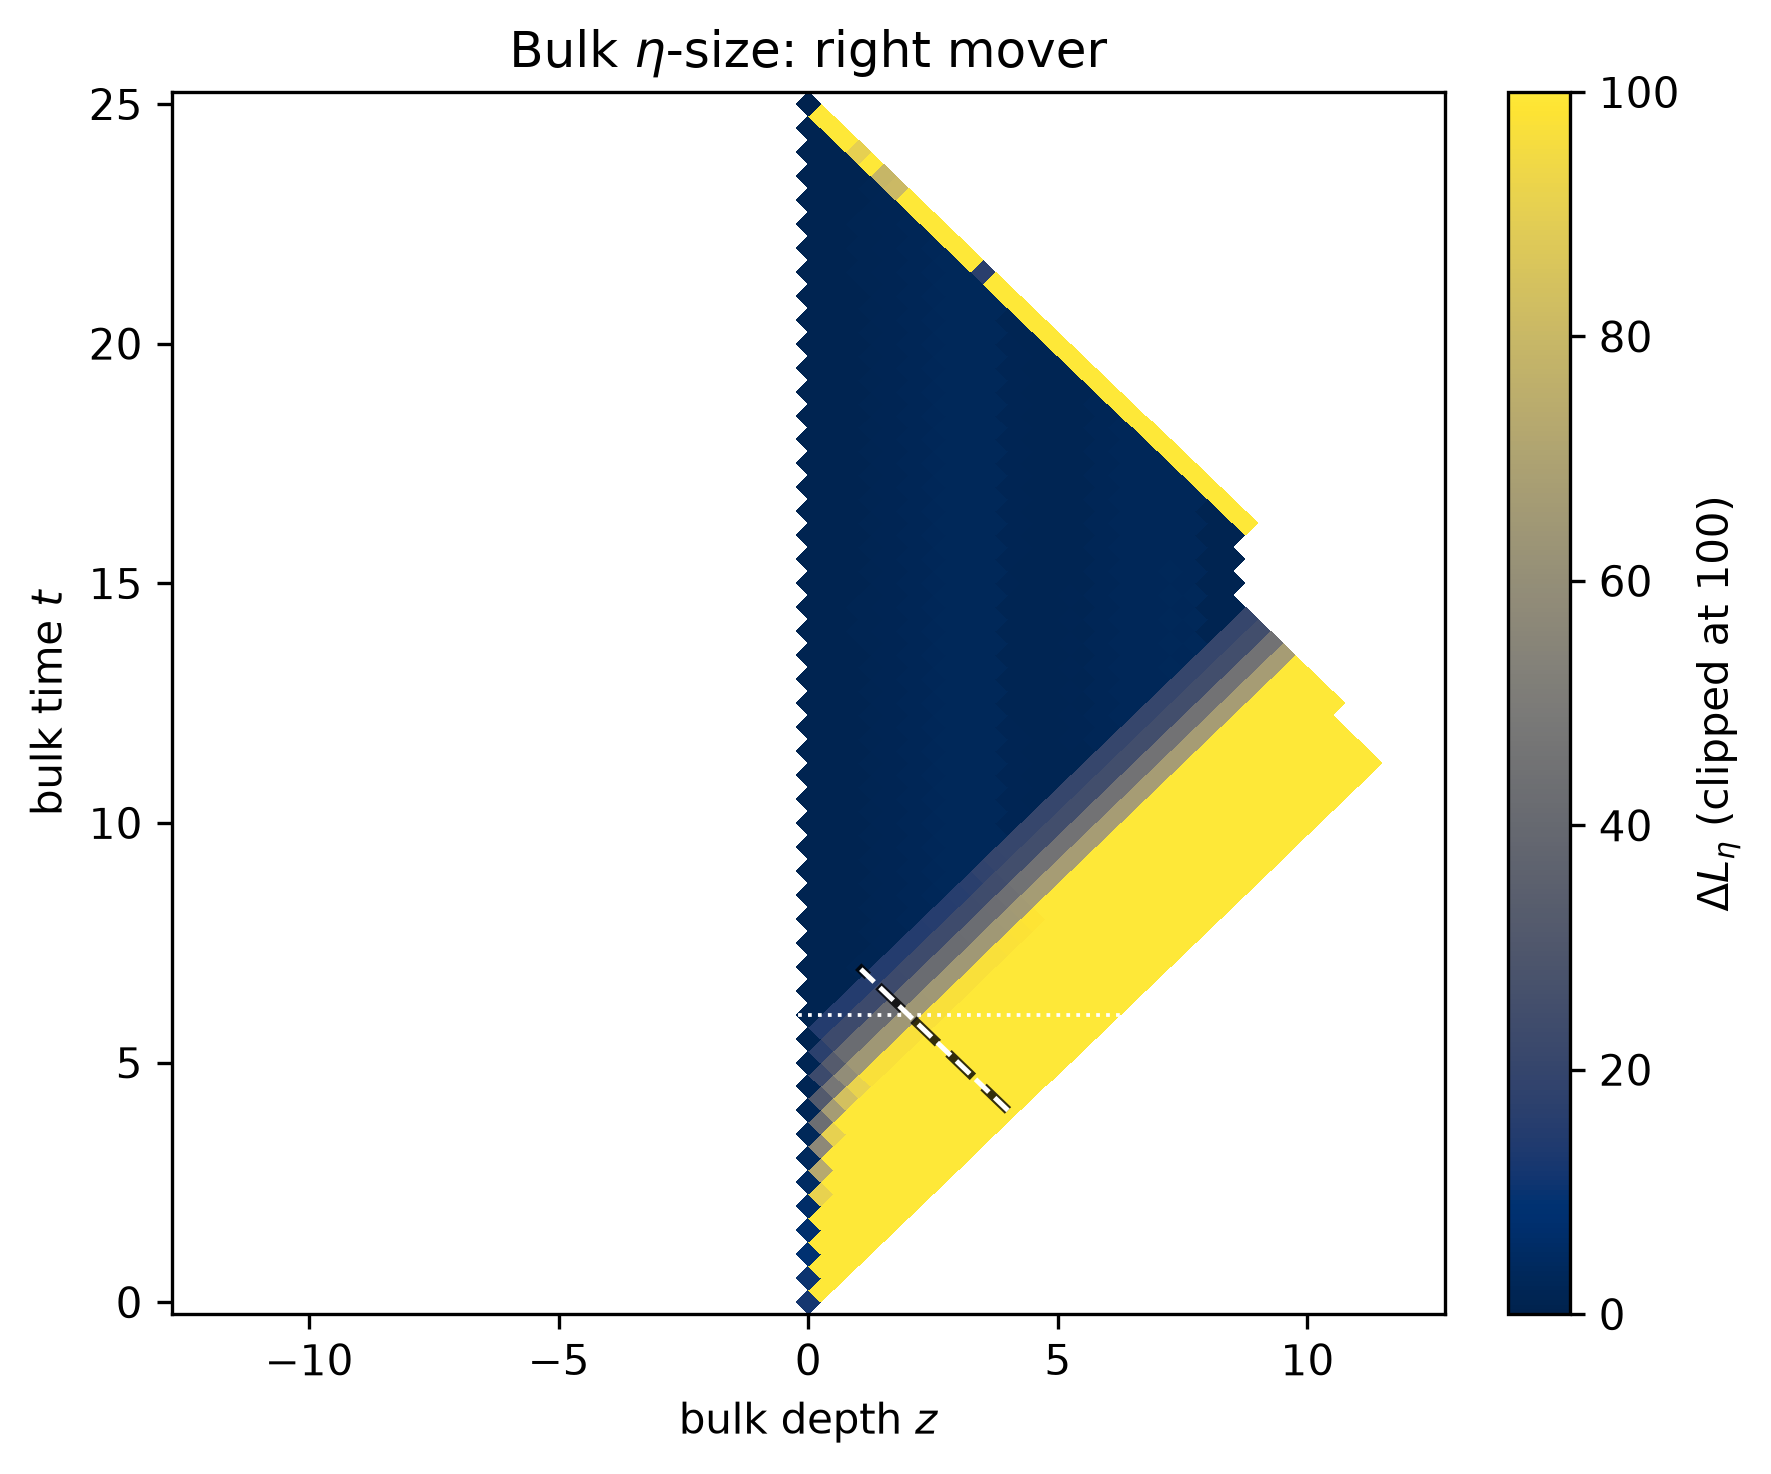
\includegraphics[width=0.49\linewidth]{fig4_eta_size_right_heatmap.png}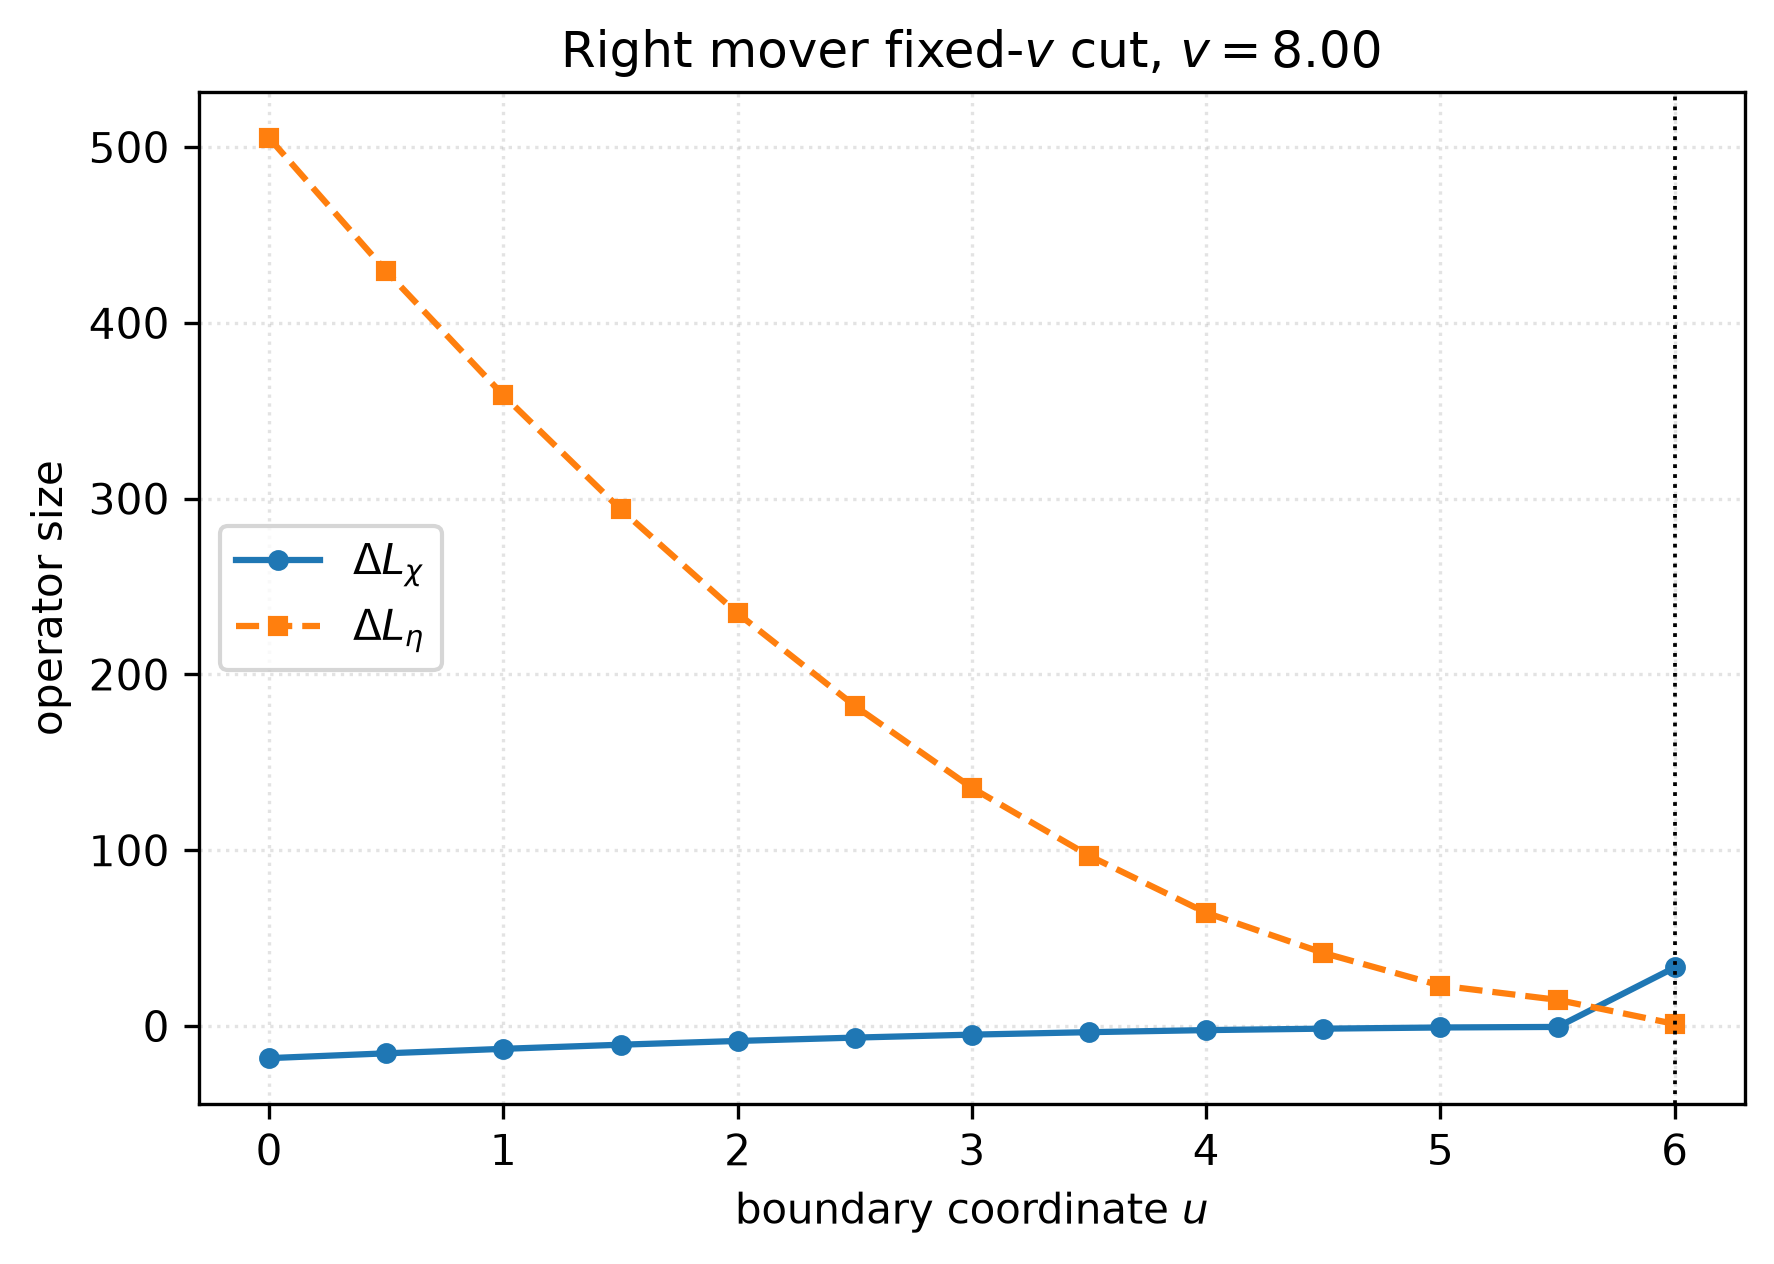
\includegraphics[width=0.49\linewidth]{fig4_right_mover_fixed_v_cut.png}
	\caption{(a) $\Delta L_\eta$ for a right-moving fermion operator $\psi_f(u,v)$. (b) $\Delta L_\eta$ and $\Delta L_\chi$ for a fixed $v$ as a function of $u$.}\label{fig:operator_size}
\end{figure}

The emergence of the past and future horizons in region II is a direct consequence of the factorized two-point function in Eq. (\ref{eq:regionII}), which shows that $\eta_a(t)$ before and after $t=t_{\rm ev}$ are almost linearly independent from each other. In the large-$N$ limit, the bulk modes at the future horizon are independent from the future simple boundary operators. In contrast, at finite $N$, unitarity of the boundary dynamics requires that no information is lost; the information carried by an infalling mode should return in a complex multi-particle excitation rather than a simple fermion mode. Our model allows us to study this return quantitatively.

In the evaporation geometry, there is a time $t_{\rm max}$ when the anti-commutator matrix $A(t,t')$ for the interval $\left[t_{\rm ev},t_{\rm max}\right]$ becomes singular. This translates to the fact that the reconstructed geometry ends at the future horizon $v=t_{\rm max}$. Consider a future-horizon infalling mode $\psi_{a,f}(u,v=t_{\rm max})$. By construction, $\left\{\psi_{a,f}(u,t_{\rm max}),\eta_b(t)\right\}=0$ for any $t\in\left(u,t_{\rm max}\right]$. Since the post-evaporation geometry has an end, all future $\eta_a(t),~t>t_{\rm max}$ only depend on $\eta_a(t),~t\in[t_{\rm ev},t_{\rm max}]$. Therefore, $\left\{\psi_{a,f}(u,t_{\rm max}),\eta_b(t)\right\}=0$ for any $t>u$. This clarifies that in the large-$N$ limit such an infalling mode is invisible in the future. Denote $\left|\Phi_\eta\right\rangle$ and $\left|\Phi_\chi\right\rangle$ as the initial states of $\eta$ and $\chi$ fermions respectively. Define
\begin{align}
	\left|\Phi(t)\right\rangle&=U(t,0)\left|\Phi_\eta\right\rangle\otimes \left|\Phi_\chi\right\rangle\\
	\left|\Psi(t)\right\rangle&=\sqrt{2}\,U(t,0)\psi_{R,f}(u,t_{\rm max})\left|\Phi_\eta\right\rangle\otimes \left|\Phi_\chi\right\rangle
\end{align}
with $U(t,0)=T\exp\left[-i\int_0^tdt'H(t')\right]$ the time evolution operator of the coupled system. $\left|\Psi(t)\right\rangle$ and $\left|\Phi(t)\right\rangle$ are the states with and without the extra infalling fermion. According to the anti-commutation computation and Wick's theorem, these two states have identical correlation functions at all future times if we choose $t>t_{\rm ev}$. (Actually it works for all $t>u$ but we will focus on $t>t_{\rm ev}$.) However, we know these two states are orthogonal (since $\left|\Phi(t)\right\rangle$ has an even number of fermions while $\left|\Psi(t)\right\rangle$ has an odd number of fermions). If we consider the presence of the additional infalling fermion as a single bit of quantum information, this information is preserved, but becomes invisible in simple correlation functions in the large-$N$ limit.

Our solution of the coupled SYK model allows us to study how the difference between these two states is detectable when we consider finite $N$ corrections. The first diagnostic is the change in the size operator
\(\hat L_\psi=i\sum_j\psi^L_j\psi^R_j\). For the infalling mode,
\begin{align}
	\Delta L_\eta(u;t_0)&=\left\langle \Psi(t_0)\right|L_\eta\left|\Psi(t_0)\right\rangle-\left\langle \Phi(t_0)\right|L_\eta\left|\Phi(t_0)\right\rangle\label{eq:DeltaLf}
\end{align}
The computation is achieved by adding a $\delta$-function perturbation to the bilinear coupling, evaluating the corresponding folded-contour four-point response, and convolving it with the bulk reconstruction kernel. The method is summarized in Methods and derived in Supplementary Text, Sec.~S4. For a pure state that entangles $\eta_{aL}$ and $\eta_{aR}$, the expectation value of $L_\eta$ has the interpretation of the operator size for the Schmidt operator, i.e. the single-sided operator whose Choi state is $\left|\Phi(t_0)\right\rangle$ or $\left|\Psi(t_0)\right\rangle$\cite{roberts2018operator,qi2019quantum}. In our model $\eta$ is entangled with $\chi$, so we can view the state of $\eta$ as an ensemble of orthogonal pure states, and $L_\eta$ is the average operator size in this ensemble. Since $L_\eta\propto N_\eta$ but $\Delta L_\eta(u;t_0)$ is of order $1$, the effect is a $\frac1{N_\eta}$ correction. The behavior of $\Delta L_{\eta,\chi}(u;t_0)$ is shown in Fig.~\ref{fig:operator_size}. We see that the operator size grows exponentially as a function of $t_{\rm ev}-u$, due to the scrambling dynamics before evaporation, and oscillates in the detection time $t_0$ due to the coupling with the bath.

\begin{figure}[htbp]
	\centering
	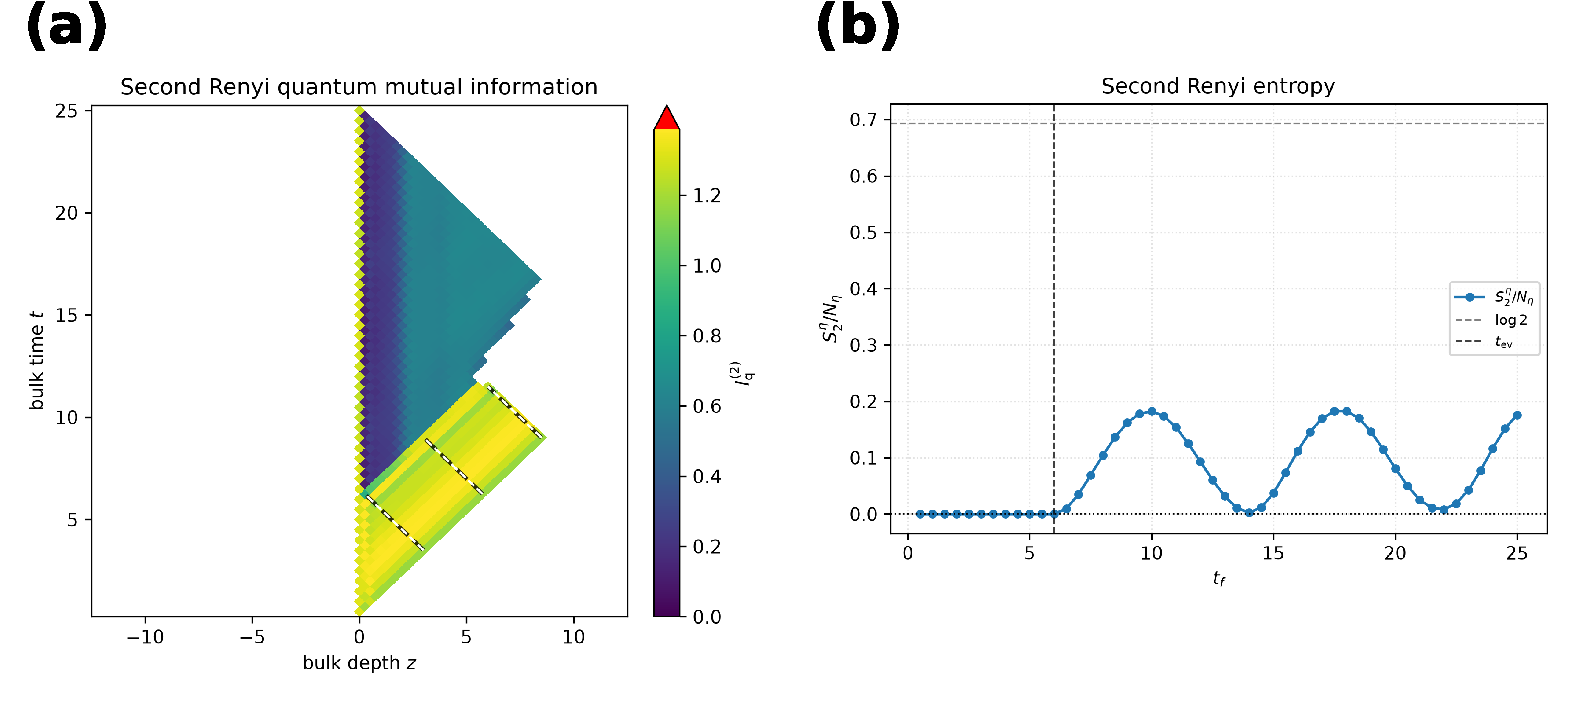
\includegraphics[width=\linewidth]{figure4_finite_p.pdf}
	\caption{Finite $p$ numerical results: (a) Renyi-$2$ mutual information of an infalling bulk fermion $\psi_f(u,v)$ with the $\eta$ system at $t_f=25$. (b) Second Renyi entropy of the $\eta$ system (without the probe particle) due to entanglement with $\chi$.}\label{fig:finite_p}
\end{figure}

In addition to the operator size, we introduce a more direct measure of the fate of the quantum information carried by the infalling fermion. For that purpose, we introduce an auxiliary fermion $P$ which is entangled with the infalling mode. This leads to the entangled state
\begin{align}
	\left|E\right\rangle=\frac1{\sqrt{2}}\left(|0\rangle_P\otimes \left|\Phi(t)\right\rangle+|1\rangle_P\otimes\left|\Psi(t)\right\rangle\right)
\end{align}
To see whether the input information is preserved in the $\eta$ or $\chi$ systems at time $t$, we can study the mutual information between $P$ and $\eta$ fermions $I(P:\eta)=S_\eta+S_P-S_{\eta P}=S_\eta+S_P-S_\chi$. The last step is true because the entire system is in a pure state. Since it is difficult to compute the von Neumann entropy, we instead study the Renyi-$2$ mutual information:
\begin{align}
		I^{(2)}(P:\eta)&=S_\eta^{(2)}+S_P^{(2)}-S_\chi^{(2)}\\
		e^{-I^{(2)}(P:\eta)}&=\frac{{\rm tr}\left(\left(\sigma_\eta+\rho_\eta\right)^2\right)}{2{\rm tr}\left(\left(\sigma_\chi+\rho_\chi\right)^2\right)}\label{eq:renyi2_MI}
\end{align}
where $\rho_\eta$ and $\sigma_\eta$ are the reduced density matrices of $\eta$ in the states $\left|\Phi(t)\right\rangle$ and $\left|\Psi(t)\right\rangle$ respectively, and similarly for $\rho_\chi,\sigma_\chi$. We have also used $S_P^{(2)}=\log 2$. Eq. (\ref{eq:renyi2_MI}) can be computed by a two-replica generalization of the Kadanoff-Baym equation, with a twisted boundary condition that swaps the two replicas of $\eta$ or $\chi$ at the final time $t$ (see Ref.~\cite{chen2020replica} for a related calculation in a different model). This method is summarized in Methods and detailed in Supplementary Text, Sec.~S5. The result is shown in Fig.~\ref{fig:finite_p}. We find that the mutual information between $P$ and $\eta$ fermions is oscillating in time. For the parameters shown, the mutual information can be close to its maximum, which means that the infalling information is mostly preserved in $\eta$ fermions. For other finite \(p\) parameter regions, \(I^{(2)}(P:\eta)\) can be small. Information moves between the $\eta$ and $\chi$ systems periodically.

The same two-replica calculation can also be used to compute the second Renyi entropy $S^{(2)}_\eta(t)=-\log{\rm tr}\left(\rho_\eta(t)^2\right)$. In the large-$p$ limit we find $S^{(2)}_\eta(t)\propto N_\eta/p$. The behavior of $S^{(2)}$ is shown in Fig.~\ref{fig:finite_p}(b). Periodically at time $t=t_{\rm ev}+nT$ with $T$ the oscillation period, the $\eta$-$\chi$ entanglement vanishes. Therefore what plays the role of Hawking radiation is mainly $\eta$ fermions, the dynamics of which becomes non-scrambling after $t_{\rm ev}$.
Part of the information goes to $\chi$ and returns to $\eta$ periodically.

\section{Interior dynamics and future directions}

In conclusion, we have proposed a new model for black hole evaporation that enables a new quantitative characterization of how information appears to be lost in the large $N$ limit from simple probes, but actually gets preserved in complex operators. The bulk $1+1$-d geometry and bulk fermions crossing the black hole horizon can be determined entirely from the boundary fermion correlation functions. Operator size and two-replica calculations allow us to directly study the fate of quantum information falling across the horizon.



We would like to emphasize that our approach can be generalized to many other models. The bulk reconstruction applies to all generalized free fields. For example, we can go beyond the probe limit and study systems with finite $s=N_\eta/(N_\eta+N_\chi)$. We can also turn on the coupling between $\eta$ and $\chi$ gradually, which provides a smoother evaporation process rather than blast freezing.

There are many open questions for future work. To obtain further information on the smoothness of the horizon and address problems such as the firewall paradox, we need to study the interior dynamics. Our bulk reconstruction algorithm only reconstructs the causal wedge of the boundary, which does not directly determine the interior dynamics. A new principle is needed to determine the interior dynamics from boundary data. Another open question is whether we can compute the entropy (or second Renyi entropy) of part of the Hawking radiation, and determine whether part of the infalling modes at the future horizon are in its entanglement island.

\section{Methods}
\label{sec:methods}

\subsection{Microscopic model and evaporation protocol}
\label{sec:methods-model}

We take \(p/2\) to be even. On one side of the doubled system the microscopic Hamiltonian is
\begin{equation}
\begin{aligned}
H[\eta,\chi;J]
&=i^{p/2}s^{-p/2}l_\eta(t)\sum_{I_p}J_{I_p}\eta_{I_p}
+i^{p/2}(1-s)^{-p/2}l_\chi(t)\sum_{K_p}J_{K_p}\chi_{K_p}\\
&\quad+i^{p/2}l_c(t)\sum_{m=1}^{p-1}\sum_{I_m,K_{p-m}}
J_{I_m;K_{p-m}}\eta_{I_m}\chi_{K_{p-m}},
\end{aligned}
\label{eq:methods-one-sided-H}
\end{equation}
where \(s=N_\eta/(N_\eta+N_\chi)\). The multi-index \(I_m=(i_1,\ldots,i_m)\) is an increasing \(m\)-tuple of \(\eta\)-indices and \(\eta_{I_m}\equiv\eta_{i_1}\cdots\eta_{i_m}\); \(K_n\) and \(\chi_{K_n}\) are defined similarly. All couplings with distinct index sets are independent Gaussian variables with zero mean and common variance
\begin{equation}
\overline{J_{I_p}^{\,2}}
=
\overline{J_{K_p}^{\,2}}
=
\overline{J_{I_m;K_{p-m}}^{\,2}}
=
\mathcal J^2\frac{2^{p-1}}{p}
\frac{(p-1)!}{(N_\eta+N_\chi)^{p-1}} .
\label{eq:methods-disorder}
\end{equation}
The left and right copies use the same disorder realization, with the reflected sign convention stated in the main text.

The sharp protocol used in the calculation is
\begin{equation}
\begin{aligned}
l_\eta(t)
&=
a\,s^{1/2}\theta(t_{\rm ev}-t)
+s^{p/2}\theta(t-t_{\rm ev}),
\\
l_\chi(t)
&=
b\,(1-s)^{1/2}\theta(t_{\rm ev}-t)
+(1-s)^{p/2}\theta(t-t_{\rm ev}),
\\
l_c(t)
&=
\theta(t-t_{\rm ev}) .
\end{aligned}
\label{eq:methods-l-protocol}
\end{equation}
For \(t<t_{\rm ev}\), \(l_c=0\), so the \(\eta\) and \(\chi\) systems are independent SYK islands of sizes \(N_\eta\) and \(N_\chi\). For \(t>t_{\rm ev}\), \(s^{-p/2}l_\eta=(1-s)^{-p/2}l_\chi=l_c=1\), so the pure and mixed \(p\)-body monomials assemble into a single SYK Hamiltonian on \(N_\eta+N_\chi\) fermions.

The bilinear couplings can be parameterized as
\begin{equation}
\begin{aligned}
\mu_\eta(t)
&=
\mu\left[
c\,\theta(-t)+\nu\,\theta(t-t_{\rm ev})
\right],
\\
\mu_\chi(t)
&=
\mu\left[
d\,\theta(t_{\rm ev}-t)+\theta(t-t_{\rm ev})
\right].
\end{aligned}
\label{eq:methods-bilinear-protocol}
\end{equation}
The evaporation protocol emphasized in the main calculation is \(a=b=1\), \(c=\nu=0\), \(d=1\), and \(\mu=\mu_0\), for which \(\mu_\eta(t)=0\) and \(\mu_\chi(t)=\mu_0\). The formation-and-evaporation extension uses \(c\neq0\), \(\nu=0\), and \(d=1\), so that the \(\eta\) bilinear is present before \(t=0\) and switched off at \(t=0\), and the \(\eta\) sector is then coupled to the bath at \(t_{\rm ev}\). Beyond this case, Supplementary Text, Sec.~S3 gives an analytical solution in the large $p$ limit for \(c=0\), \(d=1\) and \(\nu\neq0\), for which both
post-evaporation bilinear couplings are nonzero. The same formalism also allows smooth versions of these step functions.

\subsection{Large-\texorpdfstring{\(p\)}{p} two-point functions}
\label{sec:methods-large-p}

Thermofield-double initial data can be prepared by two Euclidean segments of length \(\beta/4\) on a Schwinger-Keldysh contour. The analytic figures choose the thermal \(\eta\) data and stationary coupled bath independently; the finite-\(p\) calculation uses a common preparation temperature (Supplementary Text, Secs.~S2, S3, and S5). The large-\(N\) saddle is written in terms of contour two-point functions \(G^\psi_{ab}(z_1,z_2)=-i\langle{\cal T}_{\cal C}\psi_a(z_1)\psi_b(z_2)\rangle\), where \(\psi=\eta,\chi\) and \(a,b\in\{R,L\}\) are copy indices, distinct from the protocol constants in Eq.~\eqref{eq:methods-l-protocol}. The large-\(p\) expansion separates a universal free-fermion part from order-one functions \(g^\psi_R\) and \(g^\psi_L\):
\begin{equation}
G^{\psi,>}(t_1,t_2)=-\frac{1}{2}
\left(\begin{array}{cc}
i e^{g^\psi_R(t_1,t_2)/p} & e^{g^\psi_L(t_1,t_2)/p}\\
-e^{g^\psi_L(t_1,t_2)/p} & +i e^{g^\psi_R(t_1,t_2)/p}
\end{array}\right).
\label{eq:methods-large-p-ansatz}
\end{equation}
In the general large-\(p\) equations, the interaction self-energy is determined by the kernels
\begin{equation}
\mathcal K^\psi_X
=
\alpha_\psi e^{g^\psi_X}
+l_c(t_1)l_c(t_2)
e^{s g^\eta_X+(1-s)g^\chi_X},
\qquad X=R,L ,
\label{eq:methods-large-p-kernel}
\end{equation}
where the arguments \((t_1,t_2)\) are suppressed and
\(\alpha_\eta=s^{-1}l_\eta(t_1)l_\eta(t_2)-s^{p-1}l_c(t_1)l_c(t_2)\),
\(\alpha_\chi=(1-s)^{-1}l_\chi(t_1)l_\chi(t_2)-(1-s)^{p-1}l_c(t_1)l_c(t_2)\).
Taking a second time derivative of the first-order KB equations gives
\begin{equation}
\partial_{t_1}\partial_{t_2}g^\psi_R=2\mathcal J^2\mathcal K^\psi_R,
\qquad
\partial_{t_1}\partial_{t_2}g^\psi_L=-2\mathcal J^2\mathcal K^\psi_L .
\label{eq:methods-large-p-liouville}
\end{equation}
The first-order KB equations supply the equal-time and quench matching data that are lost in this second-order form.

In the probe limit \(p\rightarrow\infty\), \(s\rightarrow0\), \(sp\rightarrow0\), \(p^2/N_\eta\rightarrow0\), the \(\chi\) sector is fixed by the traversable-wormhole solution. Defining \(r_G,\phi_G,V_G\) by
\begin{equation}
\begin{aligned}
r_G^2=e^{-2\phi_G}
&=
\frac{\mu_0}{2\mathcal J}
\left[
\sqrt{1+\left(\frac{\mu_0}{4\mathcal J}\right)^2}
-\frac{\mu_0}{4\mathcal J}
\right],
\\
V_G&=\frac{r_G}{\sqrt{1-r_G^2}},
\label{eq:methods-bath-parameters}
\end{aligned}
\end{equation}
the bath correlators are
\begin{equation}
\begin{aligned}
e^{g^\chi_R(t_1,t_2)}
&=
e^{-i\pi}
\left[
\frac{V_G}{
\sin\left(
\mathcal J V_G(t_1-t_2)-i\tanh^{-1}r_G
\right)}
\right]^2,
\\
e^{g^\chi_L(t_1,t_2)}
&=
\left[
\frac{V_G}{
\cos\left(
\mathcal J V_G(t_1-t_2)-i\tanh^{-1}r_G
\right)}
\right]^2 .
\end{aligned}
\label{eq:methods-bath-solution}
\end{equation}
Before evaporation, the \(\eta\) solution with \(\mu_\eta=0\) is
\begin{equation}
\begin{aligned}
e^{g^\eta_R(t_1,t_2)}
&=
e^{-i\pi}
\left[
\frac{\sin\vartheta}{
\sinh\left(
a\mathcal J\sin\vartheta\,(t_1-t_2)-i\vartheta
\right)}
\right]^2,
\\
e^{g^\eta_L(t_1,t_2)}
&=
\left[
\frac{\sin\vartheta}{
\cosh\left(
a\mathcal J\sin\vartheta\,(t_1+t_2)
\right)}
\right]^2,
\end{aligned}
\label{eq:methods-eta-pre}
\end{equation}
where \(\beta a\mathcal J\sin\vartheta=\pi-2\vartheta\) and $0 < \vartheta < \pi/2$. The first-order matching across \(t_{\rm ev}\) gives Eqs.~\eqref{eq:regionII} and \eqref{eq:regionIII}. The cross-region factorization in Eq.~\eqref{eq:regionII} is visible in the heatmap of the two-point function as shown in Fig.~\ref{fig:2pt_func}.
\begin{figure}[htbp]
	\centering
	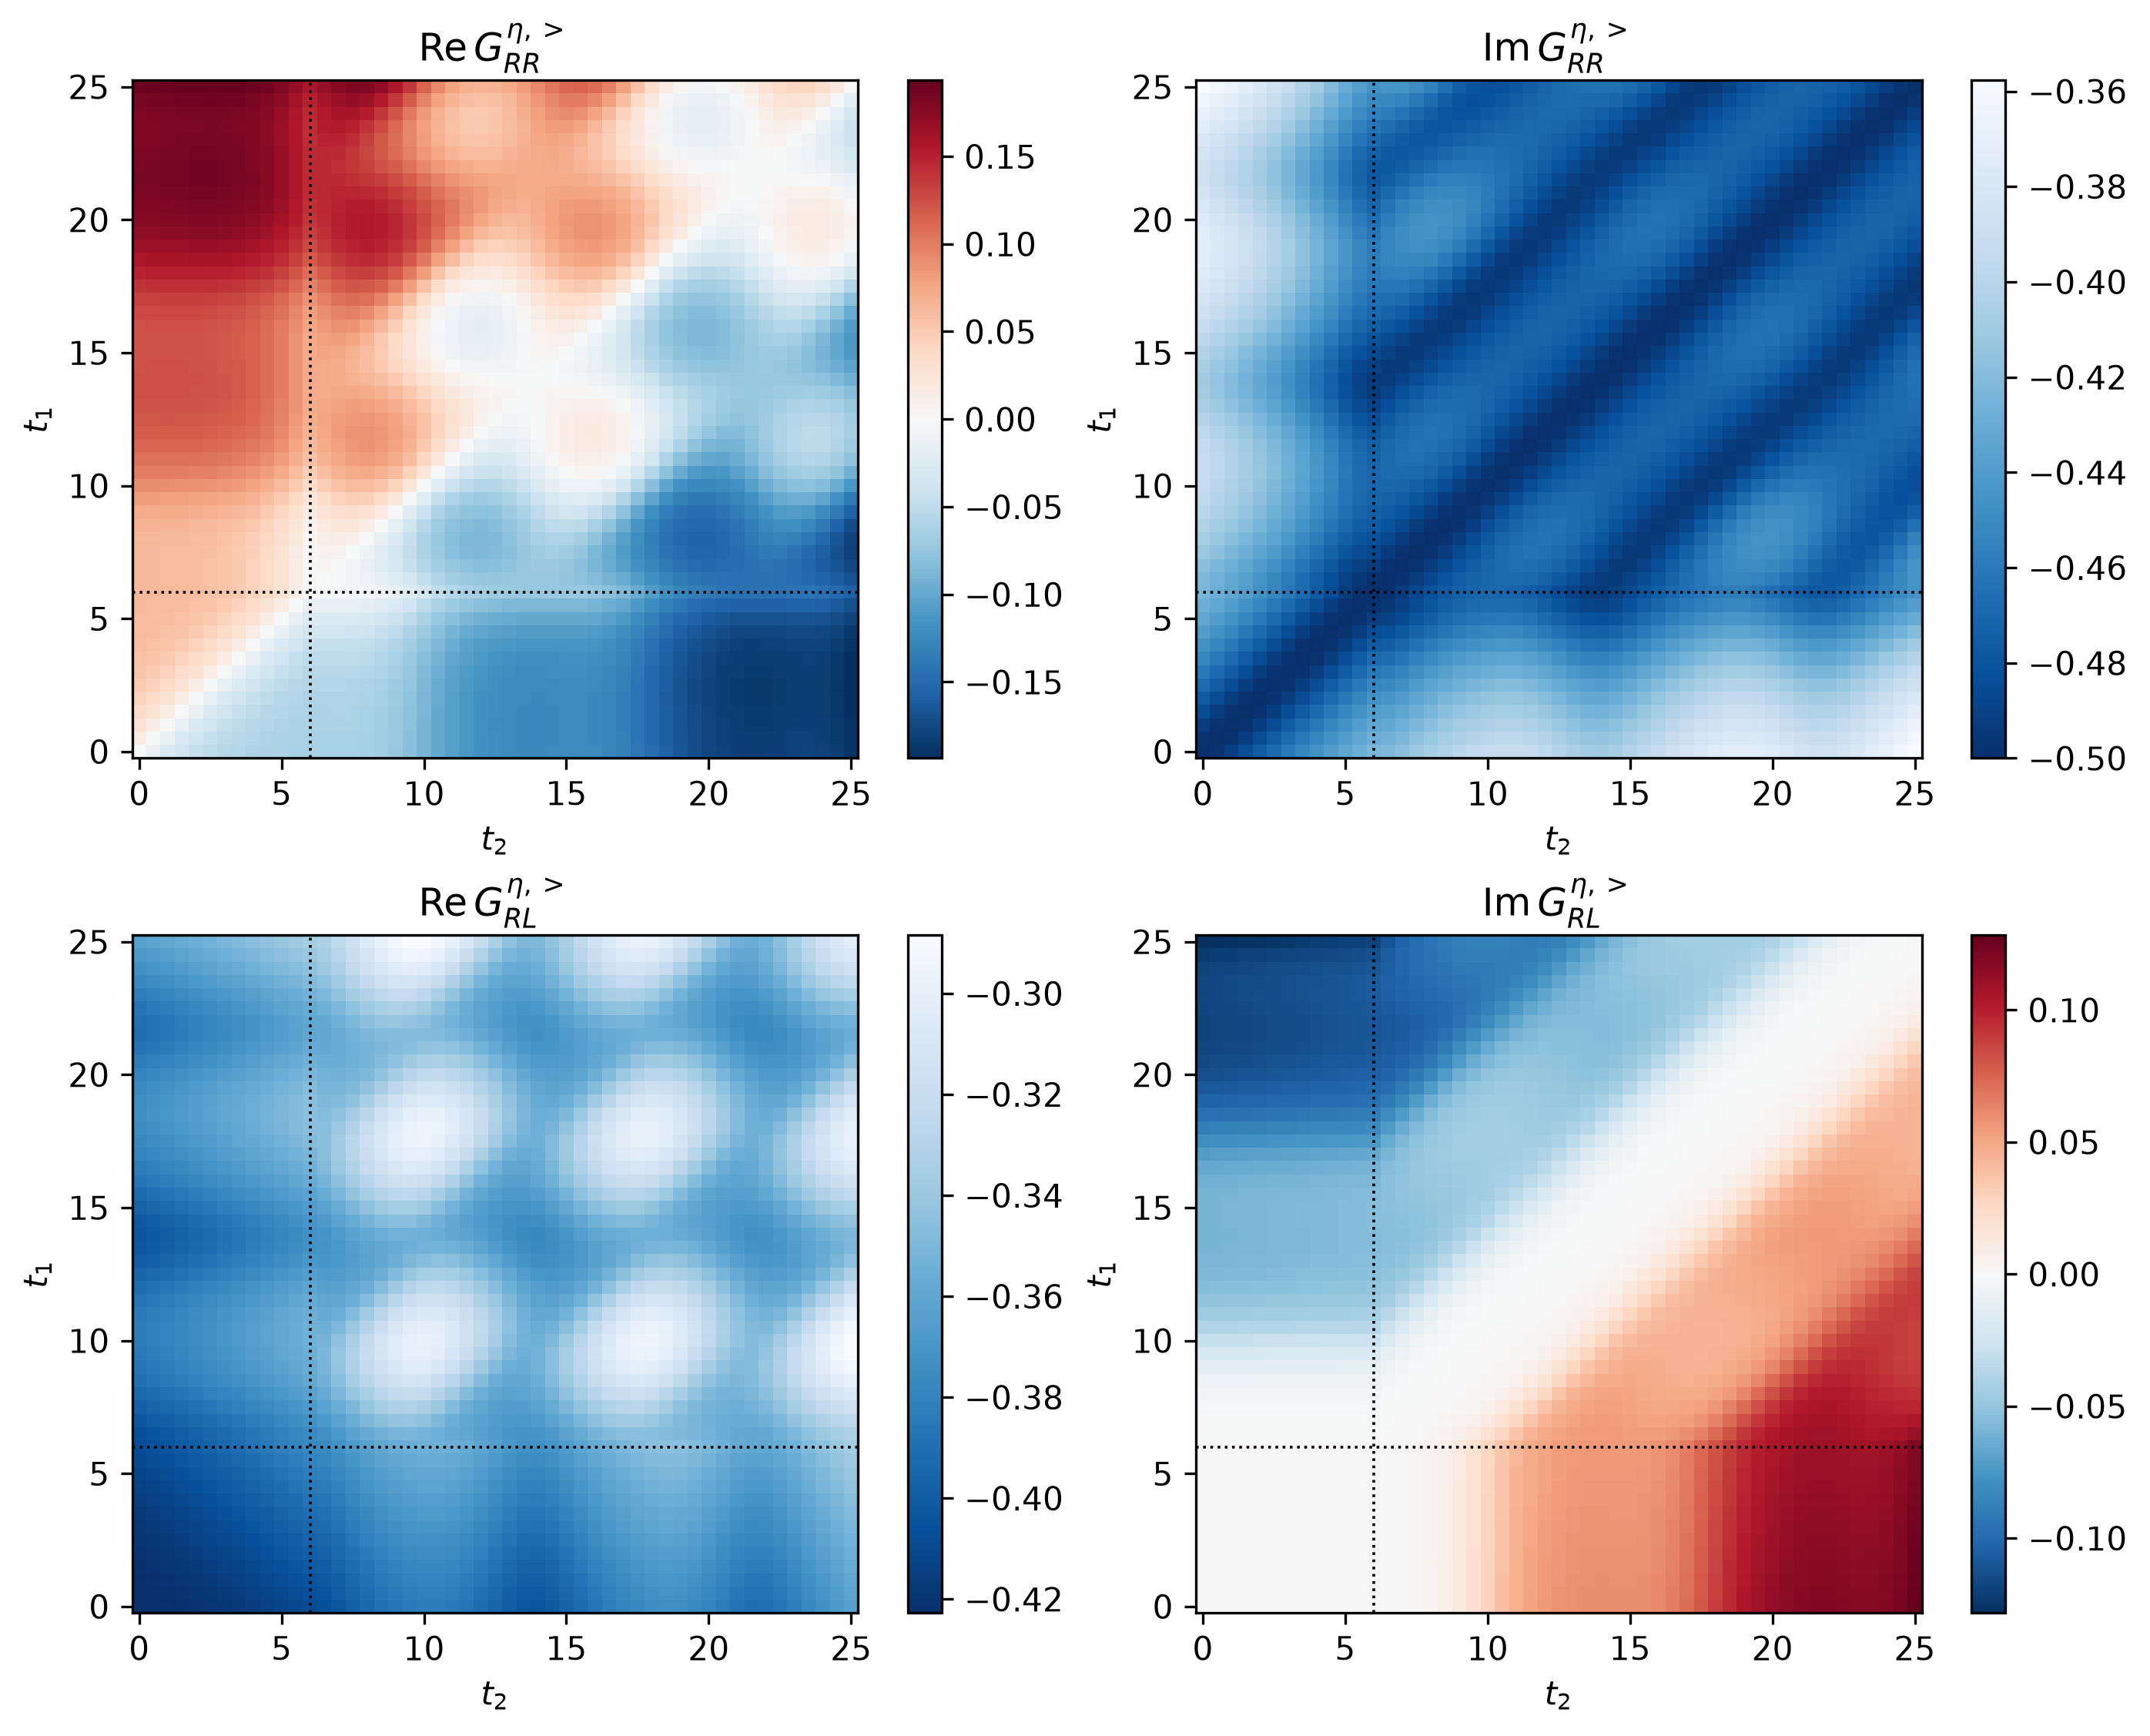
\includegraphics[width=0.60\textwidth]{fig2_two_point_heatmap.png}
	\caption{The heatmap of the two-point function in the large-\(p\) probe limit. The cross-shaped structure follows from the factorized form of the mixed-region solution.}\label{fig:2pt_func}
\end{figure}

\subsection{Bulk reconstruction algorithm}
\label{sec:methods-bulk-reconstruction}

We use the bulk reconstruction algorithm developed in Refs.~\cite{nebabu2024bulk,nebabu2026two}. For a generalized free boundary fermion, the input is the Wightman function \(C_{ab}(t_1,t_2)=\langle\eta_a(t_1)\eta_b(t_2)\rangle\). The reconstruction kernel is fixed by the anti-commutator
\begin{equation}
A_{ab}(t_1,t_2)
=
\langle\{\eta_a(t_1),\eta_b(t_2)\}\rangle
=2\,\operatorname{Re}C_{ab}(t_1,t_2).
\label{eq:methods-anticommutator}
\end{equation}
For a boundary time interval \([u,v]\), the outgoing and incoming bulk fermions are represented as linear combinations of boundary operators,
\begin{align}
\psi_{a,f(p)}(u,v)&=\int_u^v dt K_{f(p)}(u,v;t)\eta_a(t).\label{eq:HKLL_kernel}
\end{align}
After discretizing the boundary interval, write this relation as \(\psi_f=K_f\eta\) and \(\psi_p=K_p\eta\). The canonical anti-commutation relation requires
\begin{equation}
K_fAK_f^\dagger=\mathbb I,\qquad
K_pAK_p^\dagger=\mathbb I .
\label{eq:methods-kernel-orthonormal}
\end{equation}
The two kernels differ by their causal support: \(K_f\) is upper triangular in the boundary-time discretization and \(K_p\) is lower triangular. Equivalently, their inverses are obtained from Cholesky decompositions of \(A\). Once the kernels are known, the Gaussian bulk evolution between Cauchy slices \(\Sigma\) and \(\Sigma'\) is
\begin{equation}
\psi_{\Sigma'}=U_{\Sigma'\Sigma}\psi_\Sigma,
\qquad
U_{\Sigma'\Sigma}=\{\psi_{\Sigma'},\psi_\Sigma^\dagger\}.
\label{eq:methods-bulk-unitary}
\end{equation}
This construction also diagnoses topology. If \(A\) becomes singular when the boundary interval is enlarged, the bulk Hilbert space stops acquiring new orthogonal modes, which is interpreted as the end of the reconstructed geometry.

\subsection{Operator-size response}
\label{sec:methods-operator-size}

For each sector \(\psi=\eta,\chi\), define
\begin{equation}
\hat n^\psi_j
=
\left(c^\psi_j\right)^\dagger c^\psi_j
=
\frac{1}{2}
+i\psi^L_j\psi^R_j,
\qquad
\hat L_\psi=i\sum_{j=1}^{N_\psi}\psi^L_j\psi^R_j .
\label{eq:methods-size-operator}
\end{equation}
The constant \(N_\psi/2\) in the total number operator cancels in the size differences. A normalized simple boundary excitation is
\begin{equation}
\lvert\Phi_{b,j}\rangle=\sqrt{2}\,\eta^R_j(t_b)\lvert\Phi\rangle ,
\label{eq:methods-boundary-excitation}
\end{equation}
and its background-subtracted size response is
\begin{equation}
\Delta L^{\rm bdry}_\psi(t_b;t_0)
=\frac{1}{N_\eta}\sum_{j=1}^{N_\eta}
\left[
\langle\Phi_{b,j}\rvert\hat L_\psi(t_0)\lvert\Phi_{b,j}\rangle
-\langle\Phi\rvert\hat L_\psi(t_0)\lvert\Phi\rangle
\right].
\label{eq:methods-boundary-size}
\end{equation}
To compute it, introduce
\begin{equation}
f_\psi(t_1,t_2;t_0;\lambda)
=-\frac{2i}{N_\eta}\sum_{j=1}^{N_\eta}
\langle\Phi\rvert
 e^{i\lambda\hat L_\psi(t_0)/p}\eta^R_j(t_1)
 e^{-i\lambda\hat L_\psi(t_0)/p}\eta^R_j(t_2)
\lvert\Phi\rangle.
\label{eq:methods-generating-correlator}
\end{equation}
Then
\begin{equation}
\Delta L^{\rm bdry}_\psi(t_b;t_0)
=
-p\left.\partial_\lambda
f_\psi(t_b,t_b;t_0;\lambda)
\right|_{\lambda=0}.
\label{eq:methods-response-from-generating}
\end{equation}
The conjugations in Eq.~\eqref{eq:methods-generating-correlator} are represented by a folded real-time contour with a local source \(\lambda\delta(t-t_0)\hat L_\psi/p\). In the large-\(p\) variables, define
\begin{equation}
\mathfrak D_\psi(t_1,t_2;t_0)
\equiv
i\left.
\partial_\lambda
g^\eta_{R,\psi}(\widetilde t_1,t_2;t_0,\lambda)
\right|_{\lambda=0},
\label{eq:methods-D-definition}
\end{equation}
Here \(\widetilde t_1=2t_0-t_1\). The bilocal response is
\begin{equation}
\Delta L_\psi(t_1,t_2;t_0)
=
\exp\left[
\frac{g^\eta_{R,0}(t_1,t_2)}{p}
\right]
\mathfrak D_\psi(t_1,t_2;t_0),
\label{eq:methods-bilocal-size}
\end{equation}
and for a physical boundary insertion \(\Delta L^{\rm bdry}_\psi(t_b;t_0)=\mathfrak D_\psi(t_b,t_b;t_0)\). For a reconstructed infalling mode, the same bilocal response is projected with the reconstruction row \(K_f(u,t_{\rm max})\) from Eq.~\eqref{eq:HKLL_kernel}. This kernel projection gives the \(\Delta L_\eta\) and \(\Delta L_\chi\) curves in Fig.~\ref{fig:operator_size}; the explicit region-by-region response functions are in Supplementary Text, Sec.~S4.

\subsection{Two-replica KB equation and Renyi diagnostics}
\label{sec:methods-two-replica}

The Renyi-2 mutual information is computed by a two-replica version of the KB equation. Let \(\alpha,\beta\in\{1,2\}\) denote replica indices. The final-time trace over one subsystem is implemented by a signed fermionic swap between replicas. The copy labels \(a,b\) below should again be distinguished from the protocol constant \(a\) multiplying the pre-evaporation \(\eta\) interaction. In the \(\chi\)-twisted representation, the endpoint condition can be moved into a branch-dependent replica frame, producing the kernel
\begin{equation}
\Pi(z_1,z_2)=\mathsf U^\dagger(z_1)\mathsf U(z_2),
\qquad
\mathsf S=
\begin{pmatrix}
0&-1\\
1&0
\end{pmatrix},
\label{eq:methods-twist-kernel}
\end{equation}
where \(\mathsf U=\mathbf 1\) on the upper fold and \(\mathsf U=\mathsf S\) on the lower fold. In the finite-\(p\) probe limit, the two-replica \(\eta\) self-energy is

\begin{equation}
\begin{aligned}
(\Sigma^\eta_{ab})_{\alpha\beta}(z_1,z_2)
&=
(-1)^{1+p\delta_{ab}/2}
\frac{\mathcal J^2}{p}
\begin{cases}
a^2
\left[
2(G^\eta_{ab})_{\alpha\beta}
\right]^{p-1},
&z_1,z_2\in\mathcal C_<,
\\
\left[
2G^\chi_{ab}
\right]^{p-1}
\Pi_{\alpha\beta}(z_1,z_2),
&z_1,z_2\in\mathcal C_>,
\\
0,
&z_1,z_2\ {\rm on\ opposite\ sides\ of}\ t_{\rm ev},
\end{cases}
\\
&\quad
-i\epsilon_{ab}\delta_{\alpha\beta}
\frac{\mu_\eta(z_1)}{p}
\delta_{\mathcal C}(z_1,z_2).
\end{aligned}
\label{eq:methods-two-replica-self-energy}
\end{equation}

Here \(\mathcal C_<\) and \(\mathcal C_>\) denote the portions of the contour before and after evaporation. The bath correlator \(G^\chi\) is first obtained from the ordinary one-replica equation and then held fixed while solving the two-replica \(\eta\) Dyson equation. After discretizing the contour, we solve the nonlinear equation by a damped Newton-Krylov method with a GMRES inner solve.

For \(\lambda_1,\lambda_2\in\{+,-\}\), define branch-resolved contractions
\begin{equation}
C_{\alpha\beta}^{\lambda_1\lambda_2}
\equiv
2i\,
G^{(2),\eta;\chi\text{-tw}}_{RR;\alpha\beta}
(t_{b,\lambda_1},t_{b,\lambda_2};t_f),
\label{eq:methods-branch-contractions}
\end{equation}
At leading order in large \(N_\eta\), the contractions entering the mutual information are
\begin{equation}
\begin{aligned}
F_2&=C_{12}^{-+},\qquad
K_2=C_{11}^{-+},\\
F_4&=
C_{11}^{-+}C_{22}^{-+}
-C_{12}^{-+}C_{21}^{-+}
-C_{12}^{--}C_{12}^{++}.
\end{aligned}
\label{eq:methods-F-contractions}
\end{equation}
For a reconstructed infalling mode, each \(C_{\alpha\beta}^{\lambda_1\lambda_2}\) is replaced by its projection with the reconstruction row \(K_f(u,t_{\rm max})\). The Renyi-2 mutual information is then
\begin{equation}
e^{-I^{(2)}(P:\eta)}
=
\frac{1}{2}
\frac{1+2F_2+F_4}{1+2K_2+F_4}.
\label{eq:methods-MI-ratio}
\end{equation}
The same two-replica saddles give the second Renyi entropy of the \(\eta\) sector. If \(i_{\eta,\chi\text{-tw}}\) and \(i_{\eta,\rm disc}\) are the probe contributions to the statistical on-shell action in the twisted and disconnected saddles, then
\begin{equation}
\frac{S_\eta^{(2)}(t_f)}{N_\eta}
=
\operatorname{Re}\left[
i_{\eta,\chi\text{-tw}}(t_f)
-i_{\eta,\rm disc}(t_f)
\right].
\label{eq:methods-entropy-normalization}
\end{equation}
The detailed contour gluing, solver discretization, and on-shell-action formula are given in Supplementary Text, Sec.~S5.

\subsection{Parameters used in the figures}
\label{sec:methods-figure-parameters}

All numerical figures use \(\mathcal J=0.5\), \(a=1\), \(p=16\), and a real-time grid spacing \(\Delta t=0.5\). Figures~\ref{fig:bulk_geometry}, \ref{fig:operator_size}, and \ref{fig:2pt_func} use the large-\(p\) probe-limit correlators, evaluated at \(p=16\), with the \(\eta\) black-hole temperature parameter \(\beta_\eta=20\). In the convention of Eq.~\eqref{eq:methods-eta-pre}, this corresponds to \(\vartheta=0.264356318425\). The \(\eta\) bilinear coupling is zero except during the initial wormhole stage of Fig.~\ref{fig:bulk_geometry}(d--f). Figure~\ref{fig:setup} is a schematic and does not specify numerical parameter values.

\subsubsection{Bulk geometry and wavepackets (Fig.~\ref{fig:bulk_geometry}).}
The bath coupling is \(\mu_\chi=0.1\) and evaporation begins at \(t_{\rm ev}=15\). Panels (a--c) use an initially time-evolved thermofield-double state and the reconstruction interval \(0\leq t\leq80\). Panels (d--f) use the interval \(-20\leq t\leq80\), with an initial wormhole coupling \(\mu_\eta=2\mathcal J\sin^2\vartheta/\cos\vartheta\simeq0.0707285\) switched off at \(t=0\); here \(\beta_\eta\) characterizes the black-hole segment after formation. The right-moving wavepackets have initial component amplitudes \((1,0)\) and are injected at \((t,z)=(17,1)\), or \((u,v)=(16,18)\), in panel (b), and at \((t,z)=(-10,1)\), or \((u,v)=(-11,-9)\), in panel (e).

\subsubsection{Operator size and two-point functions (Figs.~\ref{fig:operator_size} and \ref{fig:2pt_func}).}
Both figures use \(\mu_\chi=0.5\), \(t_{\rm ev}=6\), and the boundary-time interval \(0\leq t\leq25\). The operator sizes in Fig.~\ref{fig:operator_size} are evaluated at detection time \(t_0=25\) for a right-moving bulk fermion. The heatmap color scale in panel (a) is clipped at \(\Delta L_\eta=100\), and the line cut in panel (b) has \(v=8\). Figure~\ref{fig:2pt_func} displays the correlators over \(0\leq t_1,t_2\leq25\).

\subsubsection{Finite-\texorpdfstring{\(p\)}{p} mutual information and entropy (Fig.~\ref{fig:finite_p}).}
The two-replica calculation uses the preparation inverse temperature \(\beta_\eta=\beta_\chi=5.7355465869\), \(\mu_\chi=0.5\), and \(t_{\rm ev}=6\). We use \(N_\beta=3\), real-time spacing \(\Delta t=0.5\), and Euclidean spacing \(\Delta\tau=\beta/(4N_\beta)\simeq0.4779622156\), so that \(\beta_{\rm grid}=4N_\beta\Delta\tau=\beta\) (Supplementary Text, Sec.~S5). Panel (a) has final measurement time \(t_f=25\) and uses the first component of the right-moving reconstructed fermion. Reconstruction kernels with norm greater than 50 are excluded; the dashed lines mark \(v=6.5,12,17.5\). Panel (b) shows \(S_\eta^{(2)}/N_\eta\) for \(t_f=0.5,1.0,\ldots,25\).

\subsection{AI assistance}
We used an AI agent (Codex) to assist in coding, checking derivations, and proofreading the manuscript.

\section*{Acknowledgements}
We would like to thank Yiming Chen and Zhenbin Yang for helpful discussions.

\section*{Funding}
This work is supported by the Simons Foundation.

% Bibliography is embedded by build.py for source submission.
% BEGIN REFERENCES
\begin{thebibliography}{10}
\expandafter\ifx\csname url\endcsname\relax
  \def\url#1{\burl{#1}}\fi
\expandafter\ifx\csname urlprefix\endcsname\relax\def\urlprefix{URL }\fi
\providecommand{\bibinfo}[2]{#2}
\providecommand{\eprint}[2][]{\url{#2}}
\providecommand{\doi}[1]{\url{https://doi.org/#1}}

\bibitem{hawking1976breakdown}
\bibinfo{author}{Hawking, S.~W.}
\newblock \bibinfo{title}{{Breakdown of predictability in gravitational
  collapse}}.
\newblock \emph{\bibinfo{journal}{Physical Review D}}
  \textbf{\bibinfo{volume}{14}}, \bibinfo{pages}{2460} (\bibinfo{year}{1976}).

\bibitem{penington2020entanglement}
\bibinfo{author}{Penington, G.}
\newblock \bibinfo{title}{{Entanglement wedge reconstruction and the
  information paradox}}.
\newblock \emph{\bibinfo{journal}{Journal of High Energy Physics}}
  \textbf{\bibinfo{volume}{2020}}, \bibinfo{pages}{2} (\bibinfo{year}{2020}).

\bibitem{penington2022replica}
\bibinfo{author}{Penington, G.}, \bibinfo{author}{Shenker, S.~H.},
  \bibinfo{author}{Stanford, D.} \& \bibinfo{author}{Yang, Z.}
\newblock \bibinfo{title}{{Replica wormholes and the black hole interior}}.
\newblock \emph{\bibinfo{journal}{Journal of High Energy Physics}}
  \textbf{\bibinfo{volume}{2022}}, \bibinfo{pages}{205} (\bibinfo{year}{2022}).

\bibitem{almheiri2019entropy}
\bibinfo{author}{Almheiri, A.}, \bibinfo{author}{Engelhardt, N.},
  \bibinfo{author}{Marolf, D.} \& \bibinfo{author}{Maxfield, H.}
\newblock \bibinfo{title}{{The entropy of bulk quantum fields and the
  entanglement wedge of an evaporating black hole}}.
\newblock \emph{\bibinfo{journal}{Journal of High Energy Physics}}
  \textbf{\bibinfo{volume}{2019}}, \bibinfo{pages}{63} (\bibinfo{year}{2019}).

\bibitem{almheiri2020replica}
\bibinfo{author}{Almheiri, A.}, \bibinfo{author}{Hartman, T.},
  \bibinfo{author}{Maldacena, J.}, \bibinfo{author}{Shaghoulian, E.} \&
  \bibinfo{author}{Tajdini, A.}
\newblock \bibinfo{title}{{Replica wormholes and the entropy of Hawking
  radiation}}.
\newblock \emph{\bibinfo{journal}{Journal of High Energy Physics}}
  \textbf{\bibinfo{volume}{2020}}, \bibinfo{pages}{13} (\bibinfo{year}{2020}).

\bibitem{almheiri2013black}
\bibinfo{author}{Almheiri, A.}, \bibinfo{author}{Marolf, D.},
  \bibinfo{author}{Polchinski, J.} \& \bibinfo{author}{Sully, J.}
\newblock \bibinfo{title}{{Black holes: complementarity or firewalls?}}
\newblock \emph{\bibinfo{journal}{Journal of High Energy Physics}}
  \textbf{\bibinfo{volume}{2013}}, \bibinfo{pages}{62} (\bibinfo{year}{2013}).

\bibitem{almheiri2013apologia}
\bibinfo{author}{Almheiri, A.}, \bibinfo{author}{Marolf, D.},
  \bibinfo{author}{Polchinski, J.}, \bibinfo{author}{Stanford, D.} \&
  \bibinfo{author}{Sully, J.}
\newblock \bibinfo{title}{{An apologia for firewalls}}.
\newblock \emph{\bibinfo{journal}{Journal of High Energy Physics}}
  \textbf{\bibinfo{volume}{2013}}, \bibinfo{pages}{1--32}
  (\bibinfo{year}{2013}).

\bibitem{maldacena1999large}
\bibinfo{author}{Maldacena, J.}
\newblock \bibinfo{title}{{The large-N limit of superconformal field theories
  and supergravity}}.
\newblock \emph{\bibinfo{journal}{International journal of theoretical
  physics}} \textbf{\bibinfo{volume}{38}}, \bibinfo{pages}{1113--1133}
  (\bibinfo{year}{1999}).

\bibitem{sachdev1993gapless}
\bibinfo{author}{Sachdev, S.} \& \bibinfo{author}{Ye, J.}
\newblock \bibinfo{title}{{Gapless spin-fluid ground state in a random quantum
  Heisenberg magnet}}.
\newblock \emph{\bibinfo{journal}{Phys. Rev. Lett.}}
  \textbf{\bibinfo{volume}{70}}, \bibinfo{pages}{3339--3342}
  (\bibinfo{year}{1993}).
\newblock \urlprefix\url{https://link.aps.org/doi/10.1103/PhysRevLett.70.3339}.

\bibitem{kitaev2015simple}
\bibinfo{author}{Kitaev, A.}
\newblock \bibinfo{title}{{A simple model of quantum holography}}.
\newblock
  \bibinfo{howpublished}{\url{https://online.kitp.ucsb.edu/online/entangled15/kitaev/};
  \url{https://online.kitp.ucsb.edu/online/entangled15/kitaev2/}}
  (\bibinfo{year}{2015}).
\newblock \bibinfo{note}{Talks at KITP, April 7 and May 27, 2015}.

\bibitem{maldacena2016remarks}
\bibinfo{author}{Maldacena, J.} \& \bibinfo{author}{Stanford, D.}
\newblock \bibinfo{title}{{Remarks on the sachdev-ye-kitaev model}}.
\newblock \emph{\bibinfo{journal}{Physical Review D}}
  \textbf{\bibinfo{volume}{94}}, \bibinfo{pages}{106002}
  (\bibinfo{year}{2016}).

\bibitem{jackiw1985lower}
\bibinfo{author}{Jackiw, R.}
\newblock \bibinfo{title}{{Lower dimensional gravity}}.
\newblock \emph{\bibinfo{journal}{Nuclear Physics B}}
  \textbf{\bibinfo{volume}{252}}, \bibinfo{pages}{343--356}
  (\bibinfo{year}{1985}).

\bibitem{teitelboim1983gravitation}
\bibinfo{author}{Teitelboim, C.}
\newblock \bibinfo{title}{{Gravitation and Hamiltonian structure in two
  spacetime dimensions}}.
\newblock \emph{\bibinfo{journal}{Physics Letters B}}
  \textbf{\bibinfo{volume}{126}}, \bibinfo{pages}{41--45}
  (\bibinfo{year}{1983}).

\bibitem{maldacena2018eternal}
\bibinfo{author}{Maldacena, J.} \& \bibinfo{author}{Qi, X.-L.}
\newblock \bibinfo{title}{{Eternal traversable wormhole}}.
\newblock \emph{\bibinfo{journal}{arXiv preprint arXiv:1804.00491}}
  (\bibinfo{year}{2018}).

\bibitem{nebabu2024bulk}
\bibinfo{author}{Nebabu, T.} \& \bibinfo{author}{Qi, X.-L.}
\newblock \bibinfo{title}{{Bulk reconstruction from generalized free fields}}.
\newblock \emph{\bibinfo{journal}{Journal of High Energy Physics}}
  \textbf{\bibinfo{volume}{2024}}, \bibinfo{pages}{1--57}
  (\bibinfo{year}{2024}).

\bibitem{zhang2019evaporation}
\bibinfo{author}{Zhang, P.}
\newblock \bibinfo{title}{{Evaporation dynamics of the Sachdev-Ye-Kitaev
  model}}.
\newblock \emph{\bibinfo{journal}{Physical Review B}}
  \textbf{\bibinfo{volume}{100}}, \bibinfo{pages}{245104}
  (\bibinfo{year}{2019}).

\bibitem{chen2020replica}
\bibinfo{author}{Chen, Y.}, \bibinfo{author}{Qi, X.-L.} \&
  \bibinfo{author}{Zhang, P.}
\newblock \bibinfo{title}{{Replica wormhole and information retrieval in the
  SYK model coupled to Majorana chains}}.
\newblock \emph{\bibinfo{journal}{Journal of High Energy Physics}}
  \textbf{\bibinfo{volume}{2020}}, \bibinfo{pages}{1--26}
  (\bibinfo{year}{2020}).

\bibitem{gaikwad2023microscopic}
\bibinfo{author}{Gaikwad, A.}, \bibinfo{author}{Kaushal, A.},
  \bibinfo{author}{Mandal, G.} \& \bibinfo{author}{Wadia, S.~R.}
\newblock \bibinfo{title}{{A microscopic model of black hole evaporation in two
  dimensions}}.
\newblock \emph{\bibinfo{journal}{Journal of High Energy Physics}}
  \textbf{\bibinfo{volume}{2023}}, \bibinfo{pages}{171} (\bibinfo{year}{2023}).

\bibitem{bragagnolo2026probing}
\bibinfo{author}{Bragagnolo, N.} \& \bibinfo{author}{Kumar, S.~P.}
\newblock \bibinfo{title}{{Probing evaporating black holes with modular flow in
  {SYK}}}.
\newblock \emph{\bibinfo{journal}{Journal of High Energy Physics}}
  \textbf{\bibinfo{volume}{2026}}, \bibinfo{pages}{185} (\bibinfo{year}{2026}).

\bibitem{lensky2021rescuing}
\bibinfo{author}{Lensky, Y.~D.} \& \bibinfo{author}{Qi, X.-L.}
\newblock \bibinfo{title}{{Rescuing a black hole in the large-q coupled SYK
  model}}.
\newblock \emph{\bibinfo{journal}{Journal of High Energy Physics}}
  \textbf{\bibinfo{volume}{2021}}, \bibinfo{pages}{116} (\bibinfo{year}{2021}).

\bibitem{nebabu2026two}
\bibinfo{author}{Nebabu, T.}, \bibinfo{author}{Qi, X.-L.},
  \bibinfo{author}{Tang, H.} \& \bibinfo{author}{Wang, H.}
\newblock \bibinfo{title}{{A Two-Point Hologram for Everything}}.
\newblock \emph{\bibinfo{journal}{arXiv preprint arXiv:2602.20295}}
  (\bibinfo{year}{2026}).

\bibitem{hamilton2006holographic}
\bibinfo{author}{Hamilton, A.}, \bibinfo{author}{Kabat, D.},
  \bibinfo{author}{Lifschytz, G.} \& \bibinfo{author}{Lowe, D.~A.}
\newblock \bibinfo{title}{{Holographic representation of local bulk
  operators}}.
\newblock \emph{\bibinfo{journal}{Physical Review D—Particles, Fields,
  Gravitation, and Cosmology}} \textbf{\bibinfo{volume}{74}},
  \bibinfo{pages}{066009} (\bibinfo{year}{2006}).

\bibitem{almheiri2025}
\bibinfo{author}{Almheiri, A.}
\newblock \bibinfo{title}{{Black Hole Disappearance}}.
\newblock \bibinfo{howpublished}{Talk at the Institute for Advanced Study}
  (\bibinfo{year}{2025}).
\newblock \urlprefix\url{https://www.youtube.com/watch?v=dVRFUeJ-orc&t=947s}.
\newblock \bibinfo{note}{Workshop on Quantum Aspects of Black Holes and
  Spacetime, December 2, 2025}.

\bibitem{roberts2018operator}
\bibinfo{author}{Roberts, D.~A.}, \bibinfo{author}{Stanford, D.} \&
  \bibinfo{author}{Streicher, A.}
\newblock \bibinfo{title}{{Operator growth in the SYK model}}.
\newblock \emph{\bibinfo{journal}{Journal of High Energy Physics}}
  \textbf{\bibinfo{volume}{2018}}, \bibinfo{pages}{1--20}
  (\bibinfo{year}{2018}).

\bibitem{qi2019quantum}
\bibinfo{author}{Qi, X.-L.} \& \bibinfo{author}{Streicher, A.}
\newblock \bibinfo{title}{{Quantum epidemiology: operator growth, thermal
  effects, and SYK}}.
\newblock \emph{\bibinfo{journal}{Journal of High Energy Physics}}
  \textbf{\bibinfo{volume}{2019}} (\bibinfo{year}{2019}).

\end{thebibliography}
% END REFERENCES
\end{document}
